


\chapter{Background and Related Work [By End of March]}
% \todo[inline]{Estimated Nb Pages: 11 - 13}
\section{Reasoning under uncertainty}
% \todo[inline]{To be read again, and check the references}
\subsection{Probabilistic and Bayesian Theory}

When assuming an objective and fully observable setting, classical binary logic can be used to assert propositions about the state of a variable as either true or false~\cite{boole1847mathematical}. For example, let $X$ be a binary variable representing the operational status of a sensor, where $X = 1$ denotes ``functional'' and $X = 0$ denotes ``faulty''.  If the internal state of the sensor is fully observable and reliable diagnostic information is available, the proposition ``the sensor is functional'' can be asserted as either true or false with certainty. However, real-world systems are rarely fully observable or deterministic. In many practical situations, the truth value of a proposition cannot be determined with certainty due to inherent variability, incomplete information, or limited observations.

Probability logic~\cite{vonNeumann1956ProbabilisticLogics,Nilsson1986ProbabilisticLogic} extends binary logic by allowing propositions to take truth values in the continuous interval $[0,1]$, thereby modeling uncertainty. 
A probability value can be interpreted as the likelihood that a proposition holds, enabling partial truth assignments and quantitative reasoning under uncertainty. The probability theory has proven highly effective for modeling randomness and variability in complex systems. However, it implicitly assumes that probability values themselves are known or can be reliably estimated from sufficient evidence.

In practice, this assumption is often violated. Probabilities are typically inferred from finite data, subjective judgment, or imperfect measurements, which introduces an additional layer of uncertainty that standard probability theory does not explicitly represent. Moreover, probability assignments are usually observer-dependent: they reflect the belief of an individual or system given its available information, rather than an objective property of the world.

Bayesian theory~\cite{gelman2013bayesian,jaynes03,Bernardo:1319894} addresses some of these challenges by treating probabilities as degrees of belief (given the knowledge) and updating them through Bayes’ rule as new evidence becomes available. Bayesian inference provides a mechanism for incorporating prior knowledge and observational data, and it is widely used in statistics and machine learning~\cite{barberBRML2011}. Nonetheless, Bayesian probability remains a single-layer uncertainty framework: uncertainty is encoded solely in probability distributions over random variables.

This limitation becomes apparent when distinguishing between uncertainty due to inherent randomness of a variable (aleatoric uncertainty) and uncertainty due to lack of knowledge or insufficient evidence (epistemic uncertainty). Reconsider the binary sensor variable $X \in \{0,1\}$, where $X=1$ denotes that the sensor is functional and $X=0$ denotes that it is faulty. An observer who has access to zero information may assign $P(X=1) = P(X=0) =0.5$, reflecting uncertainty about the sensor’s state as he has none information. Another observer may possess detailed information: for example, evidence that the sensor hardware is new and properly calibrated (supporting $X=1$), combined with recent intermittent signal dropouts or abnormal readings (supporting $X=0$). When these pieces of evidence are considered together, this observer may also assign $P(X=1)=P(X=0)=0.5$, but for a fundamentally different reason namely, the presence of conflicting evidence rather than pure ignorance.

The probability value captures uncertainty about the sensor state itself, but it does not encode uncertainty about the reliability of the probability estimate. For the first observer, the uncertainty about the probability estimate is high, while in the second case it's low. 

This example illustrates a key limitation of probabilistic and Bayesian frameworks: they cannot distinguish between uncertainty arising from randomness of the variable itself and uncertainty arising from ignorance or lack of evidence. As a result, probabilistic models conflate confidence in a probability estimate with the probability value itself. This motivates the need for extended uncertainty representations that explicitly model uncertainty about probabilities, enabling a separation between beliefs and uncertainty. Such representations form the foundation for evidence-based theories of uncertainty, including Dempster--Shafer theory and Subjective Logic, which are discussed in the following sections.
\todo[inline]{Reviewed until here}
\subsection{Second Order Probability}

A fundamental limitation of classical probability theory is that it assumes agents are always able to specify precise probability values for uncertain events. In many real-world settings, however, decision makers are uncertain not only about outcomes, but also about the probabilities themselves. This observation motivates the notion of \emph{second-order probability}, which explicitly represents uncertainty about probabilities value rather than just probabilities about events. As formalized by Baron, a second-order probability distribution \( Q(P) \) can be interpreted as the probability that the \emph{true} probability of a proposition takes the value \( P \) \cite{Baron1987}. Coming back to the example of a binary sensor state \(X \in \{0,1\}\), the second-order probability distribution \( Q(P) \) is naturally defined over the interval \([0,1]\), where \(P\) denotes the underlying probability \(P(X=1)\). In this setting, uncertainty does not only concern the sensor outcome directly, but also the value of the probability governing that outcome. A common and convenient choice for modeling such second-order uncertainty is the \emph{Beta distribution}, which is defined over \([0,1]\).

\begin{definition}[Beta Distribution]
\label{def:beta}
A random variable \(P \in [0,1]\) follows a Beta distribution with parameters \(\alpha > 0\) and \(\beta > 0\), denoted \(P \sim \mathrm{Beta}(\alpha,\beta)\), if its probability density function is given by
\[
f(P \mid \alpha, \beta) = \frac{\Gamma(\alpha+\beta)}{\Gamma(\alpha)\Gamma(\beta)} P^{\alpha-1}(1-P)^{\beta-1},
\]
where \(\Gamma(\cdot)\) is the Gamma function.
\end{definition}

The parameters \(\alpha\) and \(\beta\) can be interpreted as pseudo-counts of positive evidence (evidence supporting \(P(X=1)\)) and negative evidence (evidence supporting \(P(X=0)\)), respectively. Large values of \(\alpha+\beta\) correspond to high confidence in the estimated probability, while small values reflect substantial epistemic uncertainty. As such, the Beta distribution provides a compact and interpretable representation of second-order uncertainty over binary events.

\begin{figure}[t]
    \centering
    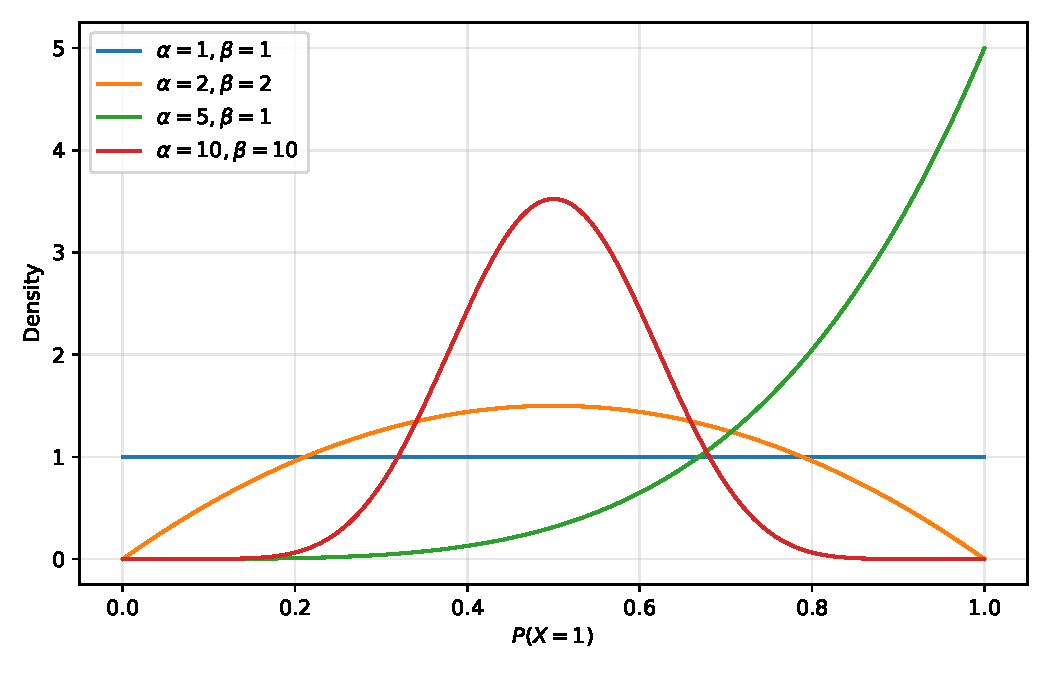
\includegraphics[width=0.65\linewidth]{img/rw/beta_distributions.pdf}
    \caption{Illustration of Beta distributions for different parameter values \((\alpha,\beta)\), showing how second-order uncertainty over \(P(X=1)\) varies from concentrated to highly uncertain.}
    \label{fig:beta_distribution}
\end{figure}

When the variable of interest can take more than two discrete values, the Beta distribution generalizes to the \emph{Dirichlet distribution}. Let \(X\) take values in a finite set \( \{x_1,\dots,x_K\} \), and let \( \mathbf{P} = (P_1,\dots,P_K) \) denote the corresponding probability vector, with \( \sum_{k=1}^{K} P_k = 1 \). Second-order uncertainty over this vector is then modeled by a Dirichlet distribution.

\begin{definition}[Dirichlet Distribution]
\label{def:dir}
A random vector \( \mathbf{P} \in \Delta^{K-1} \) follows a Dirichlet distribution with parameter vector \( \boldsymbol{\alpha} = (\alpha_1,\dots,\alpha_K) \), denoted \( \mathbf{P} \sim \mathrm{Dir}(\boldsymbol{\alpha}) \), if its density is
\[
f(\mathbf{P} \mid \boldsymbol{\alpha}) =
\frac{\Gamma\left(\sum_{k=1}^{K} \alpha_k\right)}{\prod_{k=1}^{K} \Gamma(\alpha_k)}
\prod_{k=1}^{K} P_k^{\alpha_k - 1},
\]
defined over the probability simplex \( \Delta^{K-1} \).
\end{definition}

Similarly to the Beta case, the Dirichlet parameters encode the strength and balance of evidence supporting each outcome. Uniform parameters correspond to maximal uncertainty, while peaked distributions indicate strong confidence in specific probability configurations.

\begin{figure}[t]
    \centering
    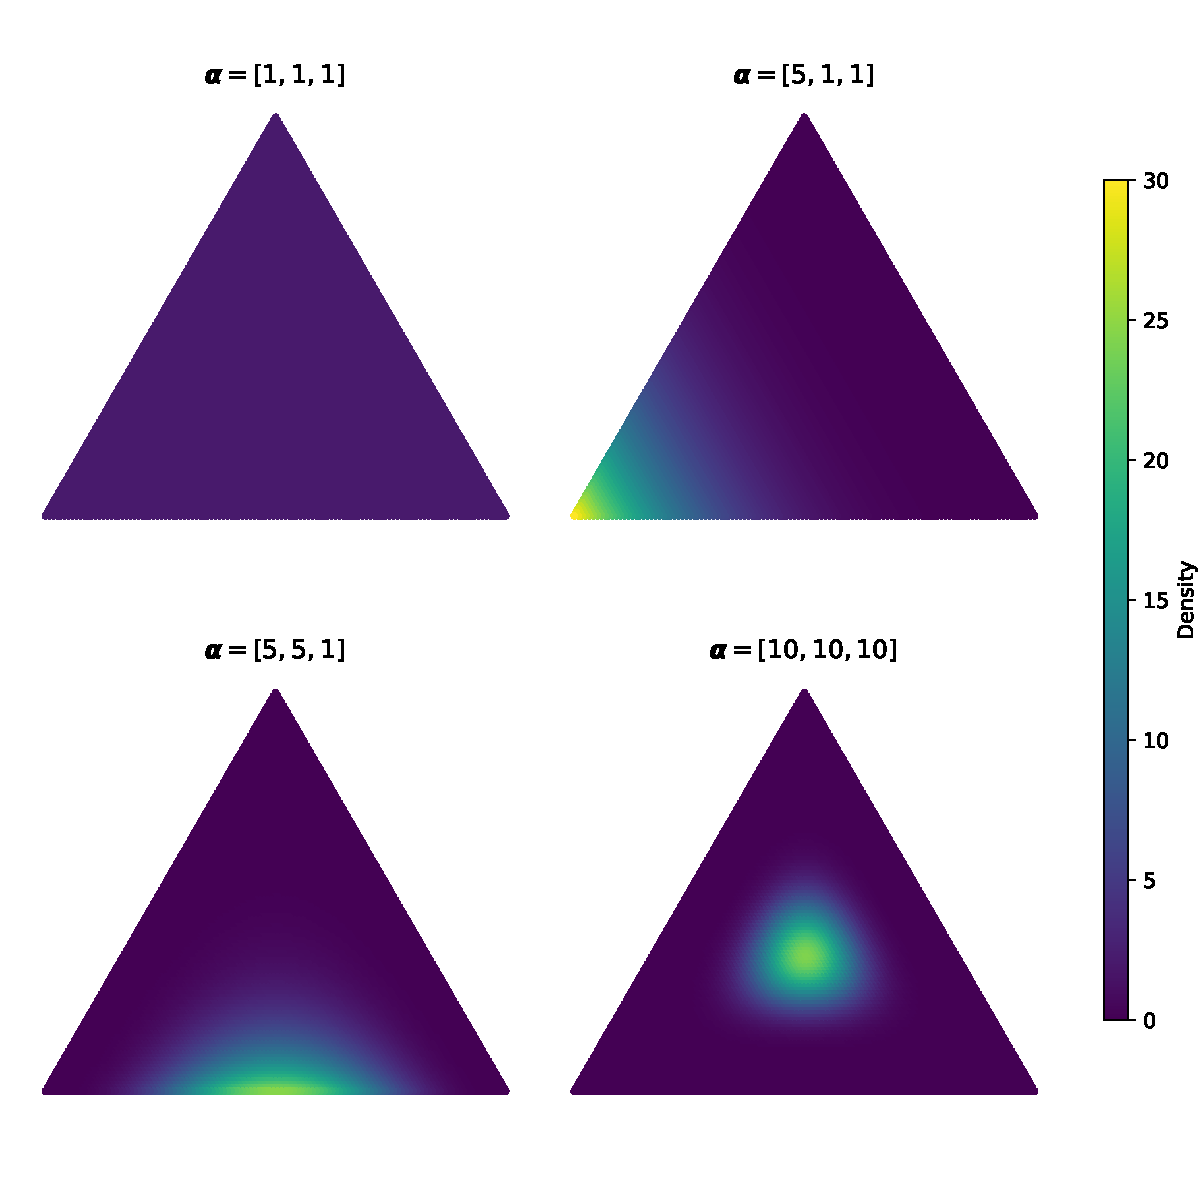
\includegraphics[width=0.65\linewidth]{img/rw/dirichlet_simplex.pdf}
    \caption{Example Dirichlet distributions over a three-class probability simplex, illustrating different degrees of second-order uncertainty.}
    \label{fig:dirichlet_distribution}
\end{figure}

This formulation allows uncertainty arising from missing, incomplete, or ambiguous evidence to be modeled explicitly, instead of being conflated with aleatoric randomness. In contrast to point-valued subjective probabilities, second-order probabilities capture the reliability of a probability assessment, a distinction that has been shown to influence human decision-making under ambiguity \cite{Baron1987}. 

Belief function theory, as introduced by Dempster and Shafer, provides an alternative framework for representing uncertainty under incomplete information. Rather than assigning probability mass exclusively to single events, belief functions distribute mass over sets of hypotheses, allowing part of the belief to remain uncommitted and explicitly representing ignorance. Dempster's rule of combination defines how independent sources of evidence may be fused within this framework. However, Baron shows that belief functions can be interpreted as a \emph{restricted special case} of second-order probability models, corresponding to strong structural constraints on the admissible forms of the distribution \( Q(P) \) \cite{Baron1987}. As a result, belief functions sacrifice expressive generality in exchange for a simplified representation of uncertainty.

This relationship is particularly relevant for uncertainty-aware trust modeling. Second-order probability provides a principled probabilistic foundation for reasoning about uncertainty in probability estimates, while belief-function-based frameworks offer practical tools for aggregating evidence and representing ignorance. These ideas directly inform later developments such as Subjective Logic, which combines second-order uncertainty representation with algebraic operators for trust discounting and fusion.

\subsection{Dempster--Shafer Theory}

\ac{DST}, also known as the theory of belief functions, was introduced to address limitations of classical probabilistic reasoning when evidence is incomplete, imprecise, or conflicting~\cite{shafer1976mathematical,beynon2000dempster}. 
Unlike Bayesian probability theory, which assigns probabilities directly to individual events, \ac{DST} allows belief to be assigned to sets of possibilities, thereby explicitly modeling uncertainty arising from lack of information.

In \ac{DST}, knowledge about a variable is represented through a basic belief assignment (BBA), which distributes belief mass over subsets of the frame of discernment rather than over single outcomes: 
\[
m: 2^{X} \rightarrow [0,1]
\]
It has two properties:
\[
m(\emptyset)=0,
\]
\[
\sum_{A\in 2^{X}} m(A)=1.
\]

This formulation enables a clear distinction between uncertainty due to ignorance and uncertainty due to randomness. In particular, belief mass assigned to composite sets represents epistemic uncertainty, while belief mass assigned to singleton sets reflects support for specific hypotheses.

A central component of \ac{DST} is Dempster’s rule of combination, which provides a mechanism for fusing evidence from multiple independent sources. 
The rule is associative, commutative, and non-idempotent~\cite{josang2012dempster}, which allows evidence to be combined incrementally and without enforcing a fixed aggregation order. 
These properties make \ac{DST} attractive for real-time and distributed applications, such as sensor fusion, where evidence arrives sequentially from multiple sources~\cite{dezert2014on}.

However, the use of Dempster’s rule requires careful consideration. Although the rule is mathematically well-defined, later studies have shown that the combination of highly conflicting sources can lead to counter-intuitive or unstable results~\cite{zadeh2013on,dezert2014on}. In cases of extreme conflict, the normalization step inherent in Dempster’s rule may amplify minor evidence and suppress uncertainty, producing misleading conclusions. As a result, \ac{DST} may become unsuitable when sources strongly disagree or when their reliability differs significantly.

Another limitation of the original \ac{DST} formulation is that it does not explicitly model trust relationships between information sources. All sources are implicitly assumed to be equally reliable, and the theory provides no native mechanism to express trust transitivity or to discount evidence based on the credibility of its origin. This limitation is particularly restrictive in multi-agent systems and distributed environments, where information is often obtained through chains of referrals and where source reliability is heterogeneous.

\subsubsection{Information Fusion and Multi-source Reasoning}
Information fusion aims to combine evidence from multiple sources in order to reduce uncertainty and improve decision quality. This problem arises in a wide range of domains, including sensor fusion, expert systems, and multi-agent systems. In multi-agent settings, agents acquire knowledge through observations or communication, and this knowledge is often represented as beliefs or belief bases~\cite{pigozzi2007aggregation}.

Early work on belief fusion relied primarily on propositional logic-based formalisms~\cite{gregoire2006logic}, and a variety of belief merging operators have been proposed to resolve inconsistencies and aggregate knowledge~\cite{konieczny2002merging,pigozzi2007aggregation,tamargo2012modeling,tran2013axiomatic}. While these approaches provide important theoretical foundations for information aggregation, they typically assume logical consistency or focus on abstract knowledge bases, limiting their applicability to uncertainty-aware reasoning in real-world systems.

\ac{DST} has been widely applied to information fusion in practical systems, particularly in sensor-based applications. For example, Munz and Dietmayer~\cite{munz2011using} employ \ac{DST} to enhance detection performance in sensor fusion systems by explicitly modeling uncertainty and combining sensory evidence. Similarly, Tang et al.~\cite{tang2017improved} use \ac{DST} to represent uncertainty in multi-sensor data before applying evidence fusion.

These works primarily address fusion within a single system, where multiple sensors act as information sources. However, they do not consider trust relationships between independent systems or agents, nor do they address the propagation of trust across information sources. As a result, while \ac{DST} provides a powerful framework for modeling epistemic uncertainty and evidence fusion, it remains limited in its ability to represent source reliability, trust transitivity, and referral-based reasoning.

These limitations motivate extensions of \ac{DST} that explicitly incorporate trust modeling and source dependency. Subjective Logic~\cite{josang2016subjective} builds upon \ac{DST} by introducing subjective opinions, trust discounting, and explicit uncertainty mass, thereby enabling trust reasoning and evidence fusion in distributed and multi-agent environments.

\section{Subjective Logic and Trust}
\ac{SL}~\cite{josang2016subjective,josang2001logic} is a formal framework for reasoning under uncertainty, grounded in probabilistic logic and the \ac{DST} of evidence~\cite{dempster1968generalization,shafer1976mathematical}. 
It extends classical and Bayesian reasoning by explicitly representing uncertainty as a first-class element of its formalism. 
In particular, \ac{SL} enables:
\begin{enumerate}
  \item the explicit representation of uncertainty as part of its fundamental building block, called a \emph{subjective opinion}, and
  \item principled reasoning about uncertainty through \emph{belief fusion}, where multiple subjective opinions are combined using well-defined operators.
\end{enumerate}

\ac{SL} models degrees of beliefs and uncertainty associated with propositions, allowing an agent to express not only what it believes, but also how confident it is in that belief. This makes \ac{SL} particularly suitable for trust modeling and reputation-based systems~\cite{LIU2011547}, as well as for uncertainty-aware assessment of machine learning systems~\cite{sensoy2018evidentialdeeplearningquantify, 10.3389/frai.2020.00054}. By explicitly distinguishing between belief supported by evidence and uncertainty due to lack or conflict of evidence, \ac{SL} addresses limitations identified in probabilistic and Bayesian frameworks.

A core concept of Subjective Logic is the notion of a \emph{subjective opinion}. In the following, we introduce subjective opinions and their formal properties, before presenting the belief fusion and trust discounting operators that enable reasoning and trust propagation in complex systems.


\subsection{Subjective Opinions} 
\label{subsec:SL_opinions}
\begin{figure}
    \centering
    \begin{subfigure}{0.49\textwidth}
    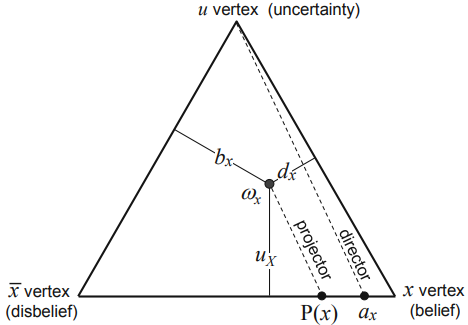
\includegraphics[width=\linewidth]{img/rw/illustration.png}
    \caption{Barycentric triangle visualisation of binomial opinion~\cite{josang2016subjective}.}
    \end{subfigure}
    \begin{subfigure}{0.49\textwidth} 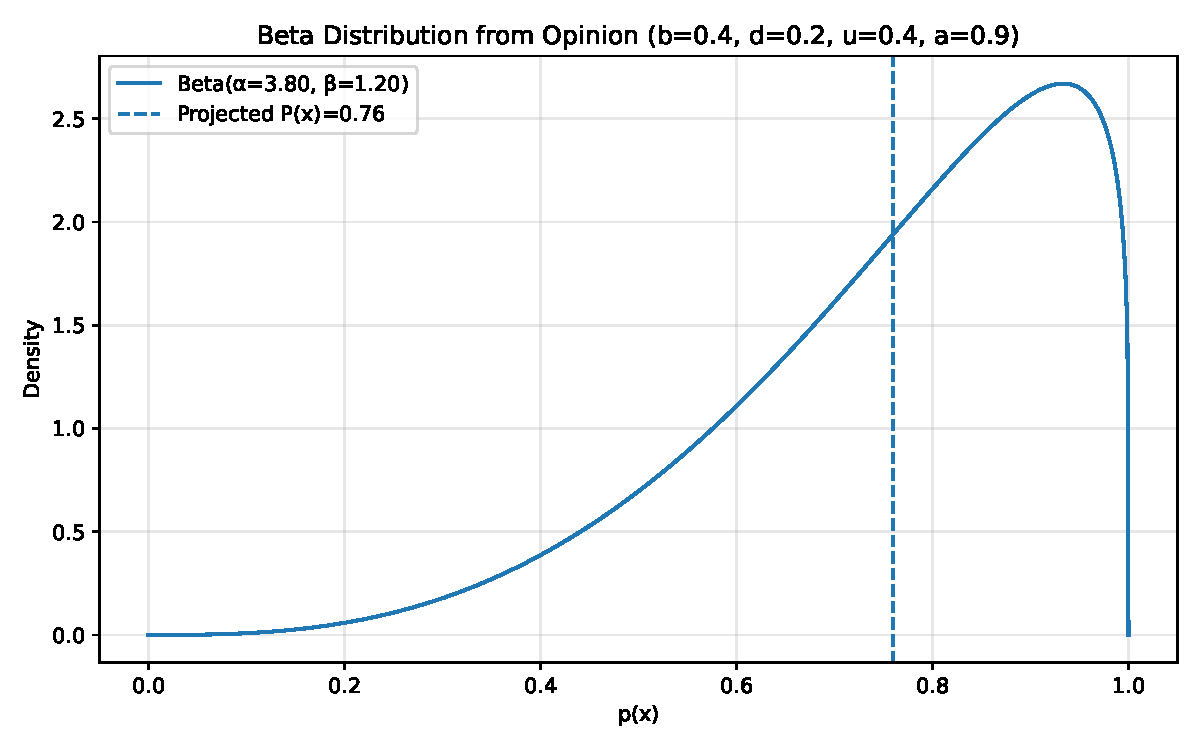
\includegraphics[width=\linewidth]{img/rw/beta_dist_map.pdf}
    \caption{Mapping to a Beta Distribution.}
    \end{subfigure}
    \caption{Binomial Opinion Visualization}
    \label{fig:bin_op_visual}
\end{figure}
Subjective opinions are the fundamental building blocks of Subjective Logic. A subjective opinion represents an agent’s belief about the state of a variable, explicitly capturing both supported belief and residual uncertainty.

Formally, a subjective opinion expresses a belief about a variable $X$ that takes values from a domain $\mathbb{X}$, also referred to as the state space. The domain $\mathbb{X}$ is assumed to be \emph{exhaustive}, meaning that it contains all possible states of $X$, and \emph{exclusive}, meaning that only one state can hold at any given time. Domains may be binary or multi-valued. A binary domain is denoted by $\mathbb{X} = \{x, \overline{x}\}$, where $\overline{x}$ denotes the complement (negation) of $x$.

The notation $\omega_X^A$ denotes a subjective opinion held by agent $A$ about variable $X$. The subscript indicates the target variable or proposition, while the superscript identifies the belief owner. When the belief owner is implicit or irrelevant, the superscript may be omitted for simplicity.

\begin{definition}[Binomial Opinion~\cite{josang2016subjective}] \label{binomial_opinion}
Let $\mathbb{X} = \{x, \overline{x}\}$ be a binary domain with binomial random variable $X \in \mathbb{X}$. 
A binomial subjective opinion about the truth of value $x$ is defined as the ordered quadruplet
\[
\omega_x = (b_x, d_x, u_x, a_x),
\]
where the additivity constraint $b_x + d_x + u_x = 1$ holds, and:
\begin{itemize}
  \item $b_x$ is the belief mass supporting $x$ being true (i.e., $X = x$),
  \item $d_x$ is the disbelief mass supporting $x$ being false (i.e., $X = \overline{x}$),
  \item $u_x$ is the uncertainty mass representing the lack of evidence,
  \item $a_x$ is the base rate, i.e., the prior probability of $x$ in the absence of evidence.
\end{itemize}
\end{definition}

A binomial opinion can be projected onto a probability value using the expected probability operator. The projected probability of $x$ is defined as:
\begin{equation} \label{eq:projected_prob}
	P(x) = b_x + a_x \cdot u_x.
\end{equation}
This projection enables compatibility with classical probabilistic reasoning, while preserving the richer internal representation of belief and uncertainty.


In the context of trust modeling, trust is typically represented as a binomial subjective opinion $(t, d, u)$, where $t$ denotes trust (belief), $d$ denotes distrust (disbelief), and $u$ represents uncertainty. 

\paragraph{Mapping to the Beta Distribution.}

A binomial subjective opinion is bijectively equivalent to a Beta probability density function (PDF). This mapping enables a probabilistic interpretation of belief masses and establishes a bridge between Subjective Logic and Bayesian statistics.

Consider a Beta distribution parameterized by $(\alpha, \beta)$ over the probability variable $p_x \in [0,1]$ (see~\cref{def:beta}) where $\alpha > 0$ and $\beta > 0$ represent evidence supporting $x$ and $\overline{x}$ respectively.

Let $r_x$ and $s_x$ denote positive and negative evidence for $x$. Under the standard non-informative prior weight $W = 2$, the mapping between a binomial opinion 
$\omega_x = (b_x, d_x, u_x, a_x)$ and a Beta distribution is given by:

\begin{equation}
b_x = \frac{r_x}{W + r_x + s_x}, 
\quad
d_x = \frac{s_x}{W + r_x + s_x},
\quad
u_x = \frac{W}{W + r_x + s_x}.
\label{eq:beta_mapping_forward}
\end{equation}

Conversely, for $u_x \neq 0$, the evidence parameters can be recovered as:

\begin{equation}
r_x = \frac{b_x W}{u_x}, 
\quad
s_x = \frac{d_x W}{u_x}.
\label{eq:beta_mapping_inverse}
\end{equation}

The projected probability of the opinion equals the expected value of the Beta distribution:
\begin{equation}
P(x) = b_x + a_x u_x
=
\mathbb{E}[p_x]
=
\frac{\alpha}{\alpha + \beta}.
\end{equation}

This bijective mapping ensures that:
\begin{itemize}
    \item High belief corresponds to concentrated density around high probability values;
    \item High uncertainty corresponds to a flat (uniform) Beta distribution;
    \item A vacuous opinion $(0,0,1,a_x)$ maps to a uniform $\mathrm{Beta}(1,1)$ distribution.
\end{itemize}

The geometric interpretation of binomial opinions is illustrated in ~\cref{fig:bin_op_visual}. The left subfigure shows the barycentric triangle representation, where belief, disbelief, and uncertainty form a 2-simplex. The right subfigure shows the equivalent Beta density, whose expectation corresponds exactly to the projected probability in \cref{eq:projected_prob}.


\begin{definition}[Multinomial Opinion~\cite{josang2016subjective}]
Let $\mathbb{X} = \{x_1, \dots, x_n\}$ be a domain with $n > 2$ mutually exclusive and exhaustive states. A multinomial opinion assigns belief masses $b_{x_i}$ to each state $x_i \in \mathbb{X}$, together with a global uncertainty mass $u$, such that
\[
\sum_{i=1}^{n} b_{x_i} + u = 1,
\]
and is complemented by a base rate distribution over $\mathbb{X}$.
\end{definition}


\begin{definition}[Hypernomial Opinion~\cite{josang2016subjective}]
A hypernomial opinion generalizes multinomial opinions by allowing belief mass to be assigned to subsets of the domain $\mathbb{X}$, enabling representation of partial or composite hypotheses.
\end{definition}

\paragraph{Mapping to the Dirichlet Distribution.}

Multinomial subjective opinions are bijectively equivalent to Dirichlet probability density functions (PDFs). This mapping generalizes the binomial–Beta correspondence and provides a Bayesian interpretation of belief masses as normalized statistical evidence.

Let $\mathbb{X} = \{x_1, \dots, x_k\}$ be a domain of cardinality $k > 2$, and let $\boldsymbol{p} = (p_1, \dots, p_k)$ be a categorical probability vector such that $\sum_{i=1}^{k} p_i = 1$.

The Dirichlet distribution parameterized by the strength vector $\boldsymbol{\alpha} = (\alpha_1, \dots, \alpha_k)$ (see \cref{def:dir}) and the parameters $\alpha_i$ represent accumulated evidence supporting outcome $x_i$.

\paragraph{Evidence Parameterization.}

Let $r_{x_i}$ denote the positive evidence supporting state $x_i$, and let $a_{x_i}$ be the base rate distribution satisfying $\sum_i a_{x_i} = 1$. 
With non-informative prior weight $W$ (typically $W = 2$), the Dirichlet strength parameters are expressed as:

\begin{equation}
\alpha_i = r_{x_i} + a_{x_i} W.
\end{equation}

The expected probability of the Dirichlet distribution is:

\begin{equation}
\mathbb{E}[p_i]
=
\frac{\alpha_i}{\sum_{j=1}^{k} \alpha_j}
=
\frac{r_{x_i} + a_{x_i} W}
{W + \sum_{j=1}^{k} r_{x_j}}.
\end{equation}

\paragraph{Bijective Mapping.}

The multinomial opinion $\omega_X = (\{b_{x_i}\}, u, \{a_{x_i}\})$ is equivalent to a Dirichlet PDF through the following mapping:

\begin{equation}
b_{x_i}
=
\frac{r_{x_i}}
{W + \sum_{j=1}^{k} r_{x_j}},
\qquad
u
=
\frac{W}
{W + \sum_{j=1}^{k} r_{x_j}}.
\label{eq:dirichlet_forward_mapping}
\end{equation}

Conversely, for $u \neq 0$:

\begin{equation}
r_{x_i}
=
\frac{W \, b_{x_i}}{u}.
\label{eq:dirichlet_inverse_mapping}
\end{equation}

Under this bijection, the projected probability of the multinomial opinion

\begin{equation}
P(x_i) = b_{x_i} + a_{x_i} u
\end{equation}

coincides exactly with the expected value of the Dirichlet distribution:

\begin{equation}
P(x_i) = \mathbb{E}[p_i].
\end{equation}

This equality ensures mathematical consistency between subjective opinions and Bayesian probability theory.

To make subjective opinions operational, Subjective Logic provides a set of reasoning operators for combining, revising, and discounting opinions. 
These operators are introduced in the following subsections.


\subsection{Belief Fusion Operators}
Belief fusion operators enable multiple subjective opinions about the same proposition to be combined into a single, aggregated opinion~(\cref{fig:sl_belief_fusion}). 
\begin{figure}[t]
    \centering
    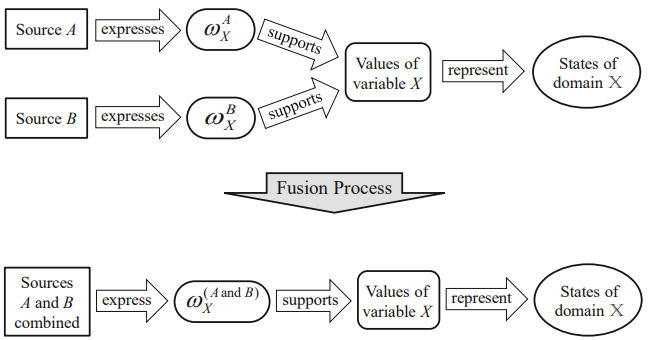
\includegraphics[width=0.6\linewidth]{img/rw/fusion_process.png}
    \caption{Belief fusion process in Subjective Logic. Two sources $A$ and $B$ express subjective opinions $\omega_X^A$ and $\omega_X^B$ about the same variable $X$. The fusion process aggregates these opinions into a single combined opinion $\omega_X^{(A \wedge B)}$, which represents the collective belief over the states of the domain of $X$~\cite{josang2016subjective}.}
    \label{fig:sl_belief_fusion}
\end{figure}

In Subjective Logic, fusion is not governed by a single universal operator; instead, multiple fusion operators are defined, each corresponding to different assumptions about the nature of the evidence sources and the fusion situation~\cite{josang2016subjective,josang2017multi}.

The need for multiple fusion operators arises from the observation that belief sources may differ in important ways, including their independence, reliability, degree of conflict, and the intended semantics of aggregation. Applying an inappropriate fusion operator can lead to misleading or counter-intuitive results. Consequently, scenario with different characteristics might need different fusion operator.

Subjective Logic defines the following principal fusion operators: \emph{constraint fusion}, \emph{cumulative fusion}, \emph{averaging fusion}, \emph{weighted fusion}, and \emph{consensus \& compromise fusion}. Each operator satisfies different algebraic properties, such as idempotence, associativity, and the existence of a neutral element, which reflect the assumptions under which the operator is valid.

\begin{figure}
    \centering
    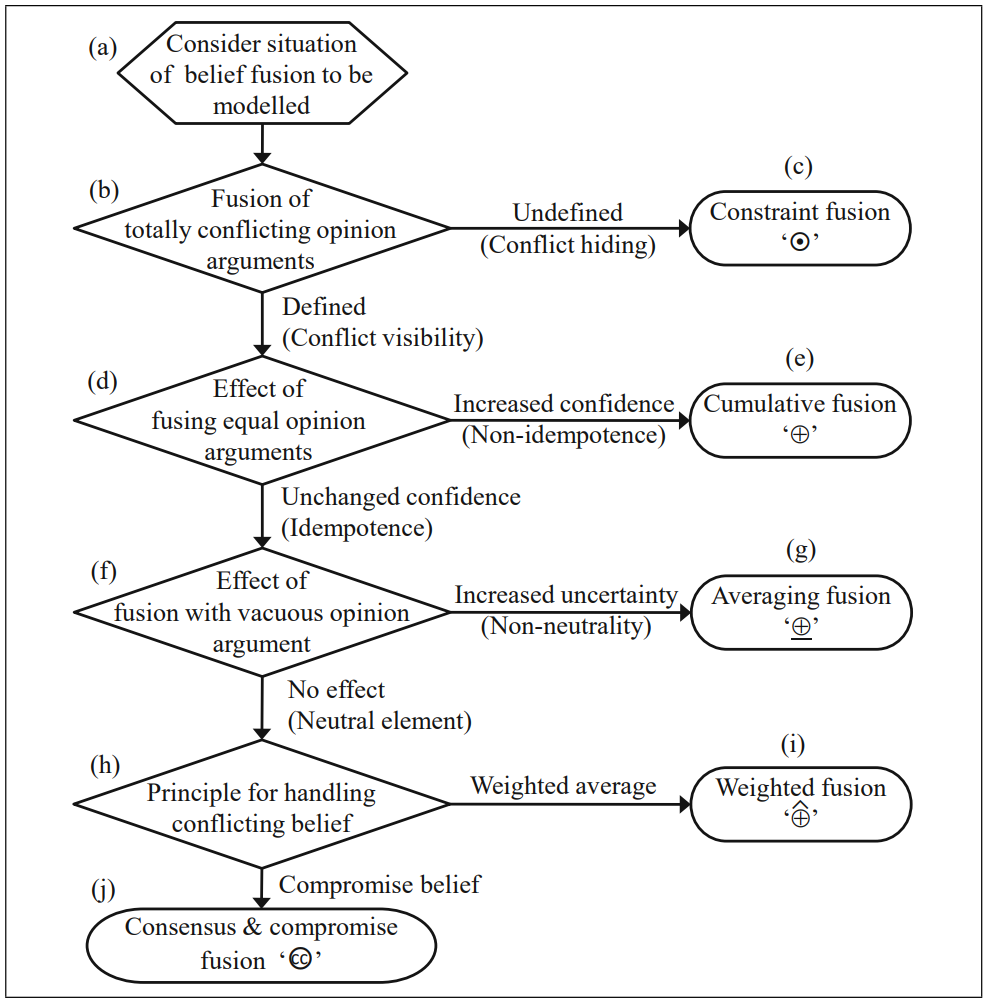
\includegraphics[width=0.65\linewidth]{img/rw/fusion_op_selection.png}
    \caption{Procedure for selecting the most adequate fusion operator}
    \label{fig:sl_fusion_selection}
\end{figure}

J{\o}sang~\cite{josang2016subjective} proposes a structured decision procedure for selecting the most appropriate fusion operator based on a sequence of semantic questions about the fusion situation. This procedure, illustrated in Figure~\ref{fig:sl_fusion_selection}, considers, among others, the following aspects:
\begin{itemize}
    \item whether totally conflicting opinions should result in an undefined outcome or a compromise,
    \item whether repeated identical opinions should increase confidence (non-idempotence) or preserve it (idempotence),
    \item whether vacuous opinions should influence the fusion result,
    \item and how conflicts between belief sources should be resolved.
\end{itemize}


\paragraph{Constraint Fusion}
Constraint fusion is appropriate when opinions are interpreted as hard or soft constraints on the possible states of a variable, and when no compromise is acceptable in the presence of total conflict. In such cases, fusion is undefined if the constraints are mutually exclusive, making conflict explicitly visible rather than hidden. This operator is particularly suitable for preference aggregation and decision-making scenarios.


\paragraph{Cumulative Fusion}
Cumulative fusion assumes that belief sources provide independent evidence about the same phenomenon. 
Under this assumption, fusing additional opinions increases the overall amount of evidence and reduces uncertainty, resulting in a non-idempotent operator. 
Cumulative fusion is commonly applied in sensor fusion and statistical evidence aggregation, where repeated observations strengthen confidence.

\paragraph{Averaging Fusion}
Averaging fusion is designed for situations where belief sources are dependent, such that combining additional opinions does not increase the total amount of evidence. This operator is idempotent and treats all opinions symmetrically, including vacuous ones. It is appropriate when opinions represent different interpretations of the same underlying observations, for example in surveys or jury deliberations.

\paragraph{Weighted Fusion}
Weighted fusion generalises averaging fusion by weighting opinions according to their confidence. More confident opinions exert greater influence on the fused result, while highly uncertain opinions contribute less. This operator is particularly relevant in expert systems, where sources may have unequal expertise or reliability, but where independence cannot be assumed.

\paragraph{Consensus \& Compromise Fusion}
Consensus \& compromise fusion explicitly separates shared belief from conflicting belief. Shared belief is preserved, while conflicting belief is transformed into uncertainty or vague belief, resulting in a compromise that reflects disagreement without artificially favouring one source. 
This operator is especially well suited for fusing hyper-opinions and for situations where preserving epistemic caution in the presence of conflict is essential.

More details about all the operators can be found in~\cref{app:SL_ops}.
\vspace{1em}

In summary, the availability of multiple fusion operators allows the analyst to align the fusion mechanism with the semantics of the application domain. This flexibility is essential for trust reasoning, where inappropriate aggregation of beliefs can lead to overconfidence or misplaced trust. In the next subsection, we introduce trust discounting operators, which explicitly model source reliability and enable trust propagation across networks of agents.


\subsection{Trust Discounting Operators} \label{subsec:TD_operators}
Trust discounting operators are a central component of Subjective Logic, enabling the propagation of trust through intermediary agents. They formalize the intuition that trust in a source should attenuate when information is relayed through other entities, thereby capturing the notion of trust transitivity.

In his foundational work~\cite{josang2016subjective}, J{\o}sang introduces two primary trust discounting operators corresponding to two distinct trust propagation scenarios: \emph{Two-Edge Path} discounting and \emph{Multi-Edge Path} discounting. These operators differ in both their semantic interpretation and their algebraic properties, and they must not be conflated.

\paragraph{Two-Edge Path Trust Discounting}
The Two-Edge Path discounting operator models trust propagation across exactly two adjacent edges: a \emph{referral trust} edge from agent $A$ to agent $B$, and a \emph{functional trust} edge from agent $B$ to a variable $X$. This situation is illustrated in Figure~\ref{fig:tdis}. The resulting discounted opinion represents the belief of $A$ about $X$, derived via its trust in $B$.

\begin{figure}[t]
\centering
    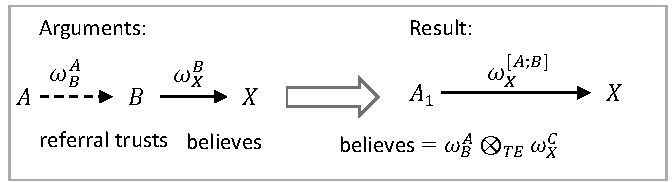
\includegraphics[width=0.7\textwidth]{img/discount/tdis.pdf}
    \caption{Trust discounting for a Two-Edge Path~\cite[Ch.~14.3]{josang2016subjective}}
    \label{fig:tdis}
\end{figure}

Formally, the Two-Edge Path discounting operator $\otimes_{TE}$ is defined as~\cite{josang2016subjective}:
\begin{equation}
    \label{equ:td}
    \omega_X^{[A;B]} = \omega^A_B \otimes_{TE} \omega^B_X =
        \begin{cases}
            b^{[A;B]}_X = P^A_B \, b^B_X,\\
            d^{[A;B]}_X = P^A_B \, d^B_X, \\
            u^{[A;B]}_X = 1 - (b^{[A;B]}_X + d^{[A;B]}_X),\\
            a^{[A;B]}_X = a^B_X,
        \end{cases}
\end{equation}
where $P^A_B$ denotes the projected probability of the referral trust opinion $\omega^A_B$ (cf. Eq.~\ref{eq:projected_prob}). 
This operator corresponds to the \emph{Base Rate Sensitive Transitivity} introduced in~\cite{josang2006exploring}.

\paragraph{Multi-Edge Path Trust Discounting}
In many real-world systems, trust is propagated across longer referral chains involving multiple intermediate agents. The Multi-Edge Path discounting operator generalizes Two-Edge Path discounting to arbitrary-length trust paths, as illustrated in Figure~\ref{fig:tdism}. Consider a trust path from agent $A_1$ to variable $X$ via intermediate agents $A_2, A_3, \dots, A_n$.

\begin{figure}[t]
    \centering
    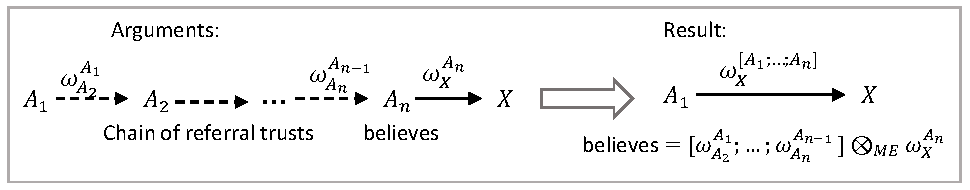
\includegraphics[width=0.8\textwidth]{img/discount/tdisM.pdf}
    \caption{Trust discounting for a Multi-Edge Path~\cite[Ch.~14.3]{josang2016subjective}}
    \label{fig:tdism}
\end{figure}

The resulting discounted opinion $\omega_X^{[A_1;\ldots;A_n]}$ is defined as:
\begin{align}
\label{equ:tdm}
    \omega_X^{[A_1;\ldots;A_n]} &=
    [\omega^{A_1}_{A_2}; \ldots; \omega^{A_{n-1}}_{A_n}] \otimes_{ME} \omega^{A_n}_X
    \\
        &=
        \begin{cases}
            b^{[A_1;\ldots;A_n]}_X = P^{A_1}_{A_n} \, b^{A_n}_X,\\
            d^{[A_1;\ldots;A_n]}_X = P^{A_1}_{A_n} \, d^{A_n}_X,\\
            u^{[A_1;\ldots;A_n]}_X = 1 - (b^{[A_1;\ldots;A_n]}_X + d^{[A_1;\ldots;A_n]}_X),\\
            a^{[A_1;\ldots;A_n]}_X = a^{A_n}_X,
        \end{cases} \notag
\end{align}
where the projected probability of the referral path is computed as
\begin{equation}
\label{equ:proj_prob}
P^{A_1}_{A_n} = \prod_{i=1}^{n-1} P^{A_i}_{A_{i+1}}.
\end{equation}

\paragraph{Discussion}
It is important to emphasize that the Two-Edge Path operator $\otimes_{TE}$ and the Multi-Edge Path operator $\otimes_{ME}$ are distinct operators with different semantics and usage constraints. In particular, both operators require that the final edge in the path corresponds to a functional trust relationship. Table~\ref{table:TD_operators} summarizes the trust discounting operators used in this work.

\begin{table}[t]
\caption{Trust discounting operators}
\centering
\begin{tabular}{|c|c|c|}
\hline
\textbf{Operator} & \textbf{Symbol} & \textbf{Application} \\ \hline
Two-Edge Path & $\otimes_{TE}$ & $\omega^A_B \otimes_{TE} \omega^B_X$ \\ \hline
Multi-Edge Path & $\otimes_{ME}$ & $[\omega^{A_1}_{A_2}; \dots; \omega^{A_{n-1}}_{A_n}] \otimes_{ME} \omega^{A_n}_X$ \\ \hline
\end{tabular}
\label{table:TD_operators}
\end{table}

\paragraph{Limitations}
J{\o}sang et al.~\cite{josang2006exploring} further investigate alternative trust transitivity (trust discounting) operators, including uncertainty-favouring and opposite-belief-favouring transitivity. However, a common limitation of these operators is that trust discounting is applied uniformly across all edges of the trust path. None of the existing operators supports selective discounting restricted to referral edges while preserving functional trust semantics. This limitation prevent to analyze some type of networks where we needs at some point to discount a referral trust opinion with another referral trust opinion. More details about that will be given in the following section, where we will see an example.

\subsection{Subjective Trust Networks} \label{subsec:SL_STN}
% \todo[inline]{Add an example using the one in the trust discounting paper. Then show limitation of current trust discounting operators}
\acp{STN} provide a graph-based formalism for modeling and reasoning about trust relationships using Subjective Logic. In an \ac{STN}, entities such as agents, systems, or sensors are represented as nodes, while directed edges encode trust relationships expressed as subjective opinions.

Formally, an \ac{STN} is represented as a directed graph $G = (V, E)$, where each node $A \in V$ corresponds to an entity, and each directed edge $(A,B) \in E$ is labeled with a binomial opinion $\omega^A_B$, representing the trust of $A$ in $B$ with respect to a given scope or context.Trust relationships may be \emph{referral trust}, expressing confidence in another agent’s reporting ability, or \emph{functional trust}, expressing confidence in the correctness of information about a specific variable.

\paragraph{Trust Inference in \acp{STN}}
To infer trust between nodes that are not directly connected, Subjective Logic relies on the trust discounting and belief fusion operators. Trust discounting is used to propagate trust along directed paths and belief fusion is used to combine multiple opinions about the same target. 

\paragraph{Trust Computation Example: Intersection Movement Assistance}
Intersection Movement Assistance (IMA) is a safety-critical application in \ac{C-ITS}, where vehicles and infrastructure components exchange information to improve road safety, traffic efficiency, and coordination. Consider the IMA scenario illustrated in Figure~\ref{fig:IMA_intersection}. Vehicle $A$ approaches an intersection and communicates via \ac{V2V} communication with vehicles $B$ and $C$. \ac{V2V} communication enables vehicles to exchange information about their state and driving behaviour~\cite{dey2016vehicle}. Vehicles $B$ and $C$ are, in turn, able to communicate with vehicle $D$, which is also approaching the intersection.

\begin{figure}[t]
    \centering
    \begin{subfigure}[b]{0.4\textwidth}
    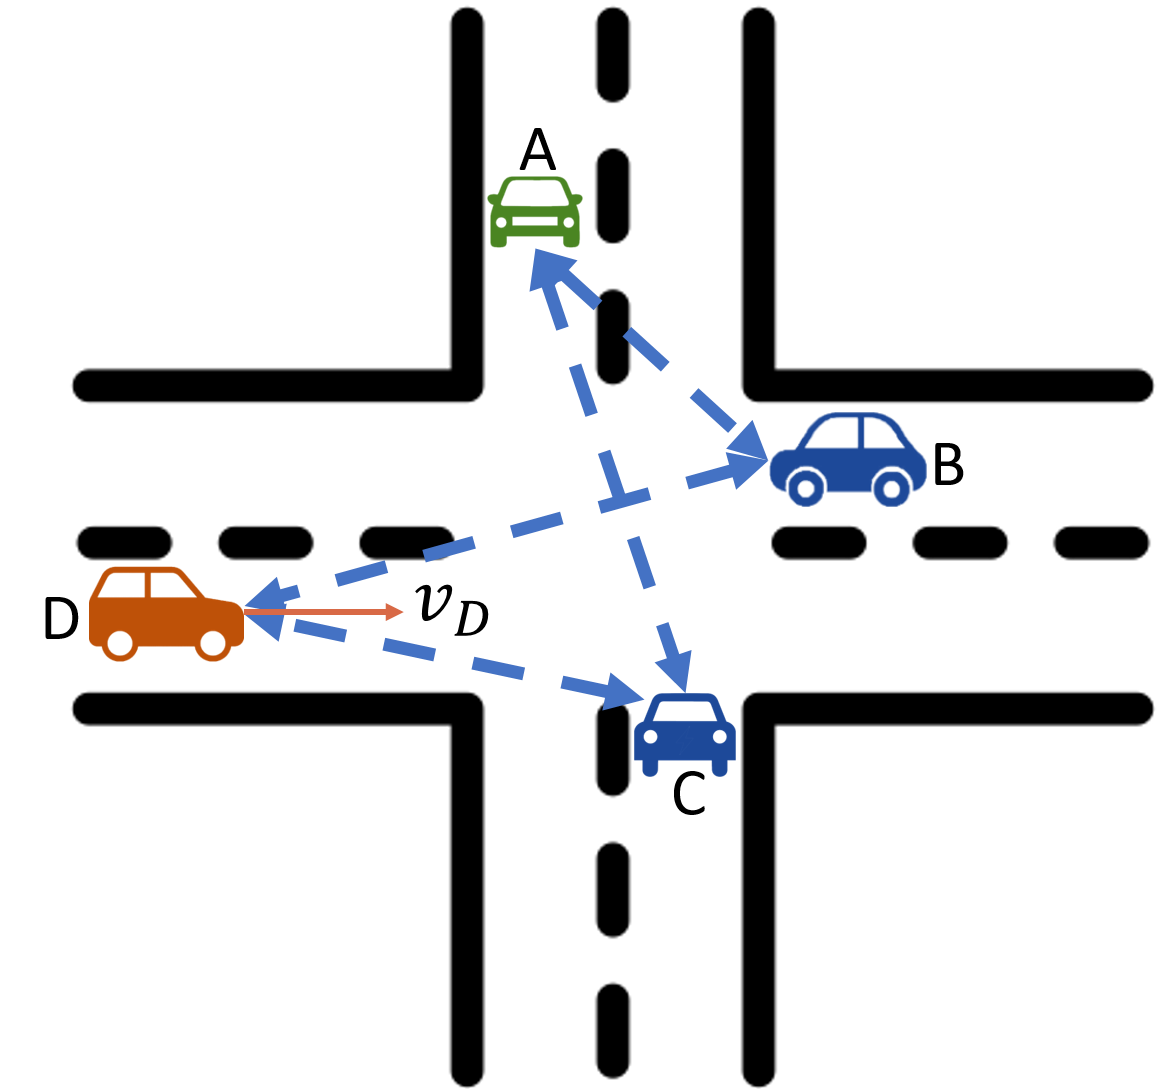
\includegraphics[width=\textwidth]{img/discount/IMA_intersection.png}
    \caption{Intersection Movement Assistance (IMA) \\ scenario}
    \label{fig:IMA_intersection}
    \end{subfigure}
    \begin{subfigure}[b]{0.59\textwidth}
    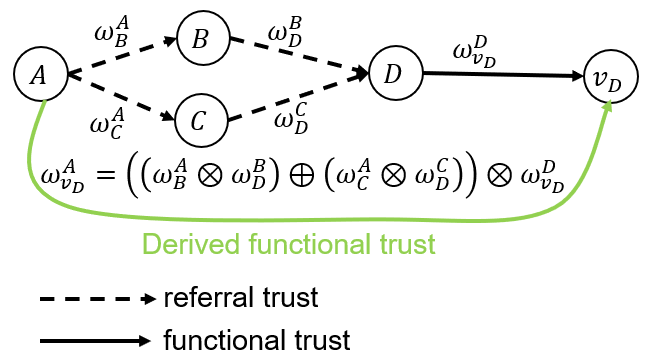
\includegraphics[width=\textwidth]{img/discount/IMA_dissertation.png}
    \caption{IMA example corresponding Subjective Trust Network}
    \label{fig:STN}
    \end{subfigure}
    \caption{}
\end{figure}

In this scenario, vehicle $A$ is interested in assessing the trustworthiness of the velocity information $v_D$ reported for vehicle $D$. Since $A$ cannot directly communicate with $D$, it cannot form a direct trust opinion about $v_D$. Instead, $A$ must rely on indirect evidence obtained through vehicles $B$ and $C$, which act as intermediaries.

This situation can be naturally modeled as a Subjective Trust Network. Vehicle $A$ holds referral trust opinions $\omega^A_B$ and $\omega^A_C$ toward vehicles $B$ and $C$, respectively, reflecting how much $A$ trusts them to provide reliable information. Vehicles $B$ and $C$ each hold functional trust opinions $\omega^B_{v_D}$ and $\omega^C_{v_D}$ regarding the velocity of vehicle $D$.

To derive its own trust opinion about $v_D$, vehicle $A$ first applies trust discounting along each referral path:
\[
\omega^{[A;B]}_{D} = \omega^A_B \otimes\omega^B_{D}, \qquad
\omega^{[A;C]}_{D} = \omega^A_C \otimes\omega^C_{D}.
\]
These discounted opinions represent $A$’s trust in \(D\) via $B$ and $C$, respectively. Since the two paths are independent, the resulting opinions are then fused to obtain a consolidated trust assessment in \(D\):
\[
\omega^A_{D} = \omega^{[A;B]}_{D} \oplus \omega^{[A;C]}_{D},
\]
where $\oplus$ denotes an appropriate belief fusion operator selected based on the semantic assumptions of the application. Finally the trust in the information \(v_D\) is:
\[
\omega^A_{v_D} = \omega^A_{D} \otimes \omega^D_{v_D} = \left( \left( \omega^A_B \otimes\omega^B_{D} \right) \oplus \left( \omega^A_C \otimes\omega^C_{D} \right)  \right) \otimes \omega^D_{v_D}
\]

This example illustrates how Subjective Trust Networks enable principled trust computation in distributed systems. Trust discounting captures the attenuation of trust across intermediaries, while belief fusion aggregates evidence from multiple independent sources. Moreover we can see that \(\omega^A_B\) and \(\omega^B_{D}\) are both referral trust opinion, therefore existing trust discounting operators cannot be used in this case. Improving trust discounting operators is then needed. \ac{SL} mechanism is essential for enabling cooperative decision-making. This motivate the need for structurally sound trust reasoning frameworks, as discussed in the following section.

\paragraph{Structural Constraints and Validity}
Trust reasoning in \acp{STN} relies on repeated applications of discounting and fusion operators along graph paths. However, not all graph structures allow computations using these operators alone. In particular, the correctness and consistency of trust inference are guaranteed when the underlying trust network satisfies the properties of a \ac{DSPG}~\cite{josang2016subjective}.

When an \ac{STN} is not a \ac{DSPG}, trust propagation may lead to ambiguous results, requiring graph transformation or restructuring before trust reasoning can be applied. Ensuring valid trust inference through structural constraints is therefore a central challenge in large-scale trust networks. We'll see more about \ac{DSPG} in the following section.


\subsection{Directed Series--Parallel Graphs (DSPG)}\label{sec:dspg}
\begin{figure}
    \centering
    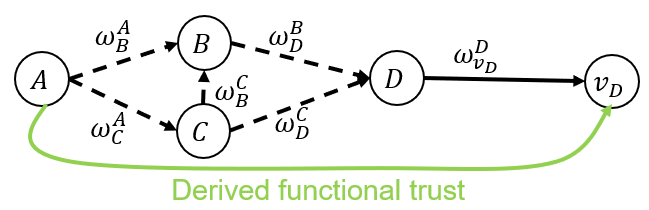
\includegraphics[width=0.5\linewidth]{img/dspg/nonDSPGIMA.png}
    \caption{Example of non DSPG \ac{STN} for the IMA usecase}
    \label{fig:non_DSPG_IMA}
\end{figure}
In \ac{TNA-SL}, \acp{DSPG} constitute the canonical graph structure that guarantees sound and unambiguous trust computation using discounting and fusion operators. As shown in the previous subsection, trust inference in Subjective Trust Networks relies on repeated applications of these operators along graph paths. However, such operations are only well defined when applied to graphs that satisfy specific structural constraints. For example, if we add a new edge from \(B\) to \(C\) (see \cref{fig:non_DSPG_IMA}) in the \ac{STN} for the IMA usecase, it becomes impossible to find the derived functional trust using trust discounting and belief fusion operators. \acp{DSPG} provide exactly the constraints the graph needs to satisfy in order to be processable.

We begin by introducing the notion of a Series--Parallel Graph, which forms the basis for \acp{DSPG}.

\begin{definition}[Series--Parallel Graph]
\label{def:spgraphs}
An SP-graph (Series--Parallel graph) is a graph that can be recursively reduced to a single edge between a source node $s$ and a sink node $t$ using the following two reduction procedures:
\begin{enumerate}[(i)]
    \item \emph{Series reduction}: replace a pair of edges incident to an intermediate node of degree~2 (excluding source and sink) with a single edge.
    \item \emph{Parallel reduction}: replace a pair of parallel edges with a single edge between their common endpoints.
\end{enumerate}
\end{definition}

Figure~\ref{fig:spgraph} illustrates a step-by-step reduction of an SP-graph. The example proceeds through four reduction stages. Reduction~1 applies the series reduction four times; Reduction~2 applies the parallel reduction twice; Reduction~3 again applies series reduction twice; and Reduction~4 applies a final parallel reduction to obtain a single edge. The existence of such a reduction sequence proves that the original graph is an SP-graph.

\begin{figure}[t]
    \centering
    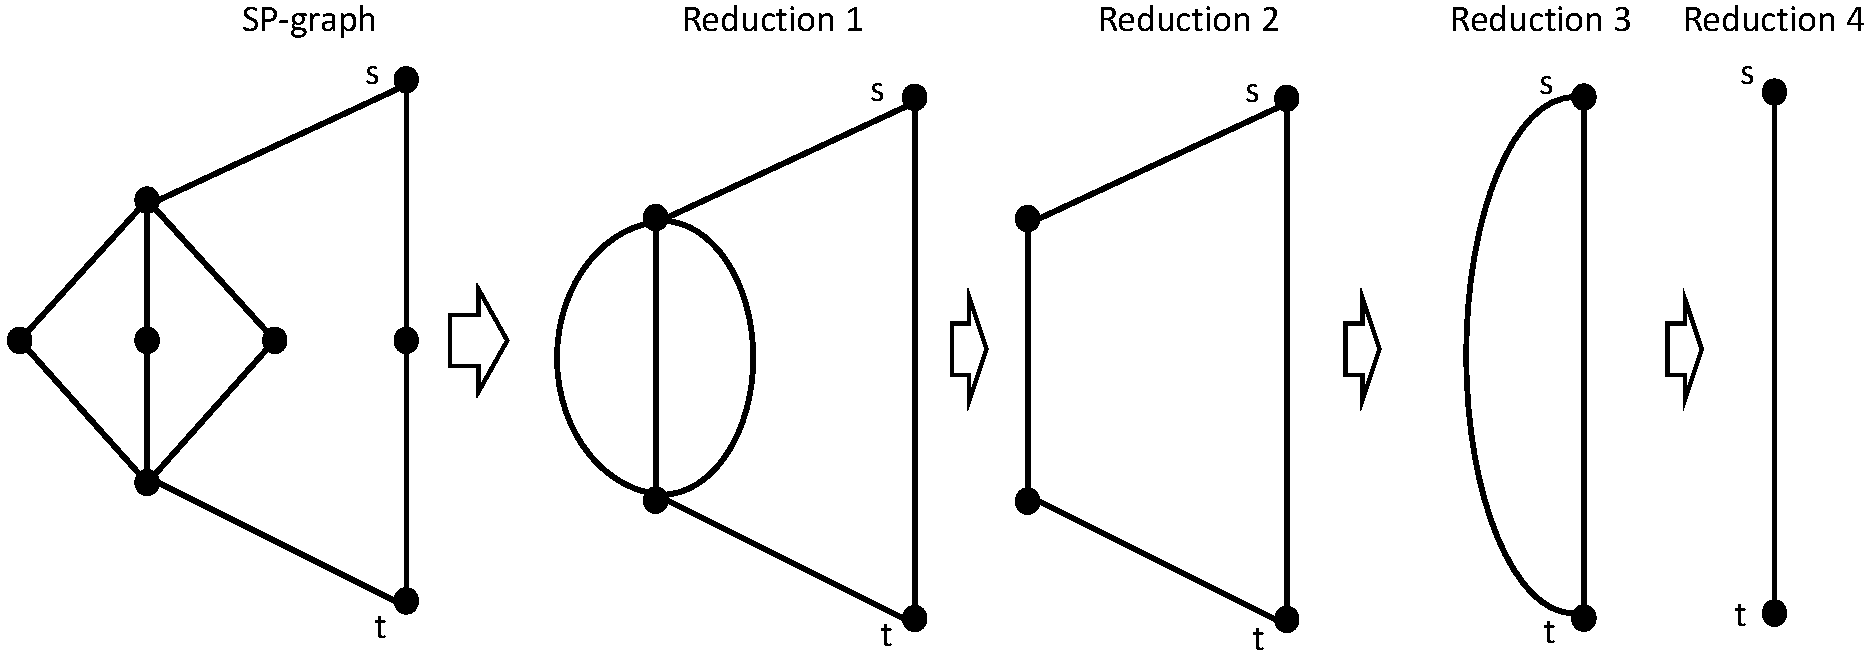
\includegraphics[width=0.6\linewidth]{img/dspg/spgraphs.pdf}
    \caption{Procedure for reducing an SP-graph into a single edge, adapted from~\cite{10.5555/3031657}}
    \label{fig:spgraph}
\end{figure}

An SP-graph that is additionally directed and acyclic, and that contains a unique source and a unique sink, is referred to as a Directed Series--Parallel Graph.

\begin{definition}[Directed Series--Parallel Graph]
A \ac{DSPG} is a directed, acyclic SP-graph composed entirely of directed paths from a unique source node to a unique sink node.
\end{definition}

These properties are essential in the context of trust reasoning. They ensure that trust propagation can be expressed exclusively through well-defined sequences of discounting (along series connections) and fusion (along parallel connections), without ambiguity or operator misuse.

\paragraph{\ac{DSPG} Analysis in Subjective Trust Networks}
In the context of Subjective Trust Networks, \ac{DSPG} analysis refers to the process of computing the derived trust opinion of a source node about a target node or variable using only Subjective Logic discounting and fusion operators. Such a computation is guaranteed to be correct and well defined if and only if the underlying trust network is a DSPG.

To formally capture the structural constraints required for \ac{DSPG} analysis, J{\o}sang introduces the following concepts~\cite{10.5555/3031657}.

\begin{definition}[Parallel Path Subnetwork (PPS)]
\label{def:pps}
A \emph{Parallel Path Subnetwork (PPS)} is a subgraph between two connected nodes $A$ and $B$ such that:
\begin{itemize}
    \item the out-degree of node $A$, denoted $outDegree(A)$, is at least~2, and
    \item the in-degree of node $B$, denoted $inDegree(B)$, is at least~2.
\end{itemize}
\end{definition}

\begin{definition}[Nesting Level (NL)]
\label{def:nl}
The nesting level of an edge in a \ac{DSPG} is defined as the number of Parallel Path Subnetworks (PPSs) to which the edge belongs.
\end{definition}

Figure~\ref{fig:ppsv} illustrates an example \ac{DSPG} and its PPS structure. 
In this example, the PPS list consists of $(A,C)$, $(C,G)$, and $(A,G)$, resulting in an edge nesting level of~2.


\begin{figure}[ht]
        \centering
        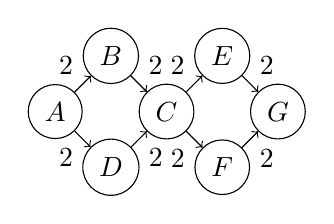
\begin{tikzpicture}[main/.style = {draw, circle}] 
        \node[main] (1) {$A$}; 
        \node[main] (2) [above right of=1] {$B$};
        \node[main] (3) [below right of=1] {$D$}; 
        \node[main] (4) [below right of=2] {$C$};
        \node[main] (5) [above right of=4]{$E$}; 
        \node[main] (6) [below right of=4] {$F$};
        \node[main] (7) [below right of=5] {$G$};
        \draw[->] (1) -- node[midway, above left]{2} (2);
        \draw[->] (1) --  node[midway, below left]{2} (3);
        \draw[->] (2) -- node[midway, above right]{2} (4);
        \draw[->] (3) -- node[midway, below right]{2} (4);
        \draw[->] (4) -- node[midway, above left]{2} (5);
        \draw[->] (4) --  node[midway, below left]{2} (6);
        \draw[->] (5) -- node[midway, above right]{2} (7);
        \draw[->] (6) -- node[midway, below right]{2}  (7);
        \end{tikzpicture}
        \caption{PPS edges NL}
        \label{fig:ppsv}
\end{figure}
Based on these definitions, J{\o}sang proposes an algorithm for computing trust over \acp{DSPG} by iteratively reducing PPSs into single edges while preserving semantic equivalence~\cite[Ch.~15.3]{10.5555/3031657}. At each reduction step, the nesting level is updated accordingly, ensuring that the order of discounting and fusion operations remains consistent with the graph structure.

\begin{figure}
    \centering
    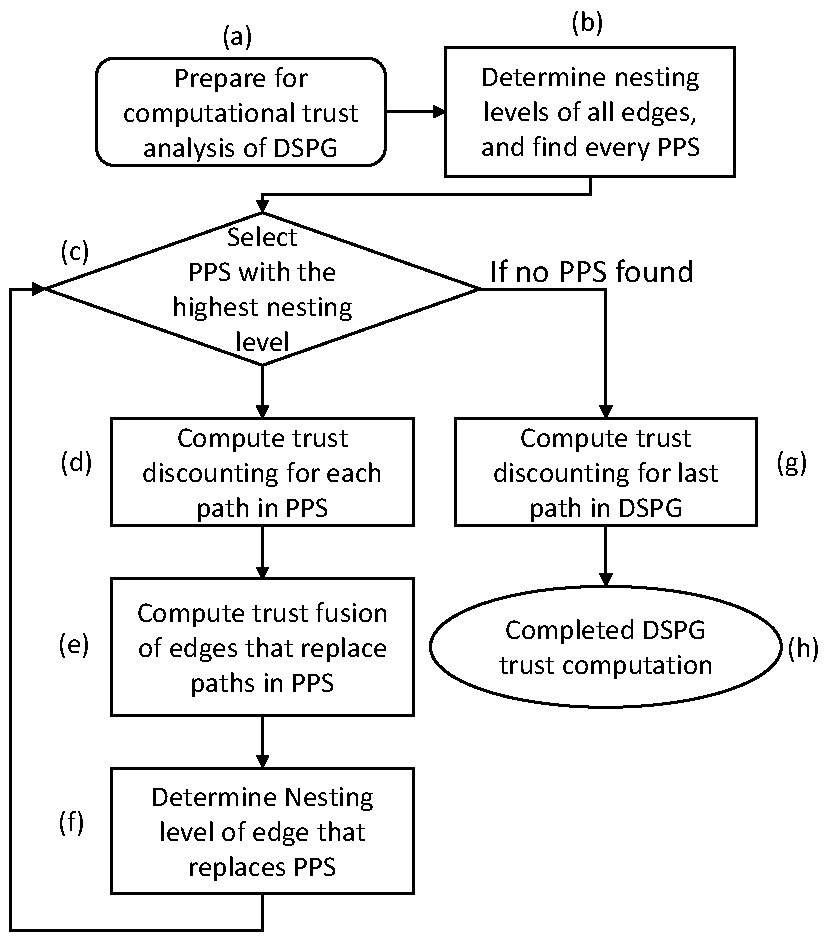
\includegraphics[width=0.5\textwidth]{img/dspg/josangSynth.pdf}
    \caption{Original \ac{DSPG} analysis algorithm by J\o{}sang \cite[Ch.15.3]{10.5555/3031657}}
    \label{fig:algsynth1}
\end{figure}


\section{Trust and Uncertainty in Neural Networks}
\subsection{Neural Networks: Background and Notation}
\label{sec:nn_background}

Neural networks are a class of parametric models widely used for function approximation in machine learning. 
They are composed of multiple layers of interconnected computational units, or neurons, which apply affine transformations followed by nonlinear activation functions. Through layered composition, neural networks can represent complex, high-dimensional mappings and have achieved state-of-the-art performance in a wide range of tasks, including image recognition, natural language processing, and control~\cite{Goodfellow-et-al-2016}.

\paragraph{Network Architecture}
We consider a feedforward neural network parameterized by
\[
\Theta = (\mathbf{W}, \mathbf{b}, f(\cdot)),
\]
where:
\begin{itemize}
    \item $\mathbf{W} = \{\mathbf{W}^{(l)}\}$ is the set of weight matrices, with $\mathbf{W}^{(l)} \in \mathbb{R}^{n_l \times n_{l-1}}$ denoting the weights connecting layer $l-1$ to layer $l$,
    \item $\mathbf{b} = \{\mathbf{b}^{(l)}\}$ is the set of bias vectors, with $\mathbf{b}^{(l)} \in \mathbb{R}^{n_l}$,
    \item $f(\cdot) = \{f^{(l)}(\cdot)\}$ is the set of activation functions, where $f^{(l)}(\cdot)$ denotes the activation applied at layer $l$.
\end{itemize}
Here, $n_l$ denotes the number of neurons in layer $l$, and the network is assumed to consist of $L$ layers.

\paragraph{Feedforward Computation}
Given an input vector $\mathbf{x} \in \mathbb{R}^{n_0}$, the network computes an output $\mathbf{y}' \in \mathbb{R}^{n_L}$ through a sequence of feedforward transformations:
\begin{align}
\label{eq:nnfeed}
\mathbf{y}' &= f_\Theta(\mathbf{x}) \\
\mathbf{y}' &= f^{(L)}\!\left(
\mathbf{W}^{(L)} 
f^{(L-1)}\!\left(
\cdots
f^{(1)}\!\left(
\mathbf{W}^{(1)} \mathbf{x} + \mathbf{b}^{(1)}
\right)
\cdots
\right)
+ \mathbf{b}^{(L)}
\right). \nonumber
\end{align}

This computation can be interpreted as the evaluation of a deterministic computational graph, where each neuron performs a fixed mathematical operation given its inputs and parameters.

\paragraph{Training Objective}
Let $\mathcal{D} = \{(\mathbf{x}_i, \mathbf{y}_i)\}_{i=1}^{N}$ denote a training dataset of input–output pairs. 
Training a neural network consists in optimizing the parameters $\Theta$ to minimize a loss function $\mathcal{L}$ over the dataset:
\[
\Theta^* = \arg\min_{\Theta} \sum_{i=1}^{N} \mathcal{L}\big(f_\Theta(\mathbf{x}_i), \mathbf{y}_i\big).
\]
This optimization is typically performed using variants of gradient descent and backpropagation~\cite{rumelhart1986learning}.

\paragraph{Determinism and Confidence}

Once trained, a standard neural network implements a \emph{deterministic mapping} from inputs to outputs.
Given an input \( x \), the network produces an output vector
\[
\mathbf{o}(x) = g(f_\theta(x)),
\]
where \( f_\theta(x) \) denotes the deterministic computation performed by the network with fixed parameters \( \theta \), and \( g(\cdot) \) is an output transformation chosen according to the task.
In classification settings, \( g \) is commonly selected so that the output components lie in the interval \( [0,1] \) and can be interpreted as class scores or probability-like values.

In practice, these outputs are often treated as estimates of posterior class probabilities,
\[
o_k(x) \approx P(y = k \mid x),
\]
and the predicted class is typically chosen as
\[
\hat{y}(x) = \arg\max_k o_k(x),
\]
with the corresponding maximum value interpreted as the model’s \emph{confidence} in its decision.

However, these confidence values primarily reflect \emph{relative activation strengths} induced by the learned parameters rather than an explicit representation of uncertainty or evidential support.
They arise from deterministic transformations of the input and do not, by themselves, encode information about ambiguity, data scarcity, or model ignorance.

For example, in a binary classification task, output vectors such as \( (0.9, 0.1) \) and \( (0.6, 0.4) \) are commonly interpreted as highly confident and weakly confident predictions, respectively.
Nevertheless, both outputs may result from equally deterministic computations and do not necessarily differ in terms of the quality or reliability of the underlying evidence.

As a consequence, neural networks may assign high confidence to predictions made on \emph{out-of-distribution inputs}, \emph{ambiguous samples}, or data affected by \emph{noise, bias, or corruption}.
In such situations, large output values do not reliably correspond to predictive accuracy or trustworthiness.

This observation highlights a fundamental limitation of confidence estimates derived from standard neural network outputs and motivates the need for \emph{additional mechanisms to quantify uncertainty and assess reliability} beyond raw model confidence, which is the focus of the following section.

\subsection{Uncertainty and Trust Quantification in Neural Networks}
\label{sec:uq_nn}

Quantifying uncertainty in neural networks has become a central research topic, particularly in safety-critical domains such as healthcare, autonomous driving, finance, and industrial automation. In these settings, incorrect yet confident predictions can lead to severe consequences. A representative example is data poisoning, where systematically mislabeled samples are present in both the training and test datasets. In such cases, a model may achieve high accuracy, precision, and recall on the poisoned test set, creating an illusion of reliability despite having learned erroneous or harmful patterns. This highlights a fundamental limitation of standard performance metrics: while they assess predictive accuracy, they fail to capture deeper aspects of predictive reliability and trustworthiness.

Uncertainty Quantification (UQ) seeks to address this limitation by explicitly modeling uncertainty associated with neural network predictions. Rather than producing point estimates alone, UQ methods aim to characterize the full predictive distribution, enabling models to express confidence, ambiguity, and ignorance in a principled manner. Recent surveys provide comprehensive overviews of UQ techniques in deep learning and emphasize their importance for robust and trustworthy AI systems~\cite{Gawlikowski2023,ABDAR2021243}.

In the literature, uncertainty in neural networks is commonly categorized into \emph{aleatoric} and \emph{epistemic} uncertainty~\cite{kendall2017uncertainties,Gawlikowski2023}.

\subsubsection{Aleatoric and Epistemic Uncertainty}

Aleatoric uncertainty captures irreducible uncertainty inherent in the data-generating process, such as sensor noise, measurement errors, or intrinsic variability in observations. This type of uncertainty cannot be reduced by collecting additional data of the same type and is typically modeled as observation noise. Aleatoric uncertainty is often further divided into \emph{homoscedastic} uncertainty, which is constant across inputs, and \emph{heteroscedastic} uncertainty, which varies as a function of the input~\cite{kendall2017uncertainties}.

Epistemic uncertainty, by contrast, arises from limited knowledge about the model parameters or structure. It reflects uncertainty due to insufficient, biased, or unrepresentative training data, as well as uncertainty induced by model misspecification~\cite{neal1996bayesian}. Unlike aleatoric uncertainty, epistemic uncertainty can, in principle, be reduced by acquiring additional data or improving model expressiveness. Figure~\ref{fig:aleatoric_epistemic} provides an illustrative distinction between the two: aleatoric uncertainty manifests as noise around the underlying function, while epistemic uncertainty appears in regions where data are sparse or absent.

This distinction is critical in safety-critical applications. High aleatoric uncertainty may indicate that a task is inherently ambiguous, whereas high epistemic uncertainty suggests that the model is extrapolating beyond its knowledge and that its predictions should be treated with caution.

Beyond this dichotomy, recent work highlights the importance of \emph{distributional uncertainty}, which arises when test samples differ significantly from the training distribution, as in out-of-distribution (OOD) or domain-shift scenarios~\cite{hendrycks2018baselinedetectingmisclassifiedoutofdistribution,ovadia2019trustmodelsuncertaintyevaluating,Gawlikowski2023}. Explicitly modeling distributional uncertainty is essential for detecting unfamiliar inputs and avoiding confident predictions in unsupported regions of the input space.

\subsubsection{Bayesian, Ensemble, and Sampling-Based Approaches}

Foundational approaches to UQ are grounded in Bayesian inference. Bayesian Neural Networks (BNNs) place probability distributions over network parameters and infer posterior distributions given observed data~\cite{neal1996bayesian,blundell2015weightuncertaintyneuralnetworks}. This formulation provides a principled representation of epistemic uncertainty by marginalizing predictions over plausible parameter configurations. However, exact Bayesian inference is computationally intractable for modern deep architectures.

To address this limitation, several approximate inference techniques have been proposed Bayes by Backprop~\cite{blundell2015weightuncertaintyneuralnetworks} employs variational inference to learn approximate posterior distributions over network weights. Monte Carlo dropout interprets dropout at inference time as a variational Bayesian approximation~\cite{gal2016dropoutbayesianapproximationrepresenting}. By performing multiple stochastic forward passes, MC dropout yields predictive distributions that approximate epistemic uncertainty with relatively low computational overhead, and has been widely adopted due to its simplicity.

Deep ensemble methods provide an alternative, non-Bayesian approach to uncertainty estimation~\cite{lakshminarayanan2017simplescalablepredictiveuncertainty}. 
By training multiple models independently and aggregating their predictions, ensembles capture predictive variability and often achieve strong empirical performance in terms of calibration and OOD detection~\cite{ovadia2019trustmodelsuncertaintyevaluating}. However, ensembles are computationally expensive and lack a unified probabilistic interpretation, which complicates the semantic interpretation of their uncertainty estimates.

More structured approaches explicitly model predictive uncertainty using latent variables or hierarchical formulations. For example, latent variable models enable the decomposition of predictive uncertainty into aleatoric and epistemic components~\cite{pmlr-v80-depeweg18a}. These methods have proven particularly useful in active learning and reinforcement learning, where uncertainty-aware decision making can improve sample efficiency and robustness.

\subsubsection{Deterministic and Distributional Uncertainty Methods}

In addition to Bayesian and sampling-based approaches, several deterministic methods aim to estimate uncertainty using a single forward pass.
Softmax confidence scores and predictive entropy are commonly used as simple uncertainty proxies, but they are known to be poorly calibrated and unreliable under distribution shift~\cite{guo2017calibrationmodernneuralnetworks}.

More advanced deterministic methods explicitly model uncertainty at the output level. Prior Networks~\cite{malinin2018predictiveuncertaintyestimationprior} parameterizes Dirichlet distributions over class probabilities, enabling the model to distinguish between data uncertainty and distributional uncertainty. Such methods have shown promise in OOD detection and risk-sensitive classification, although their effectiveness depends strongly on training objectives and data assumptions~\cite{Gawlikowski2023}.

\subsubsection{Calibration and Reliability Challenges}

Despite substantial progress, accurately estimating and calibrating uncertainty in deep neural networks remains challenging. Large-scale empirical studies report frequent over-confidence or under-confidence, particularly under dataset shift, adversarial perturbations, or real-world deployment conditions~\cite{ovadia2019trustmodelsuncertaintyevaluating,begoli2019need}. In medical AI, miscalibrated confidence estimates have been linked to critical decision errors and patient safety risks~\cite{begoli2019need,wolf2025medvlms}.

Calibration refers to the agreement between predicted confidence levels and empirical outcome frequencies. Common evaluation tools include reliability diagrams and scalar metrics such as Expected Calibration Error (ECE) and its variants~\cite{Naeini_Cooper_Hauskrecht_2015}. Post-hoc calibration methods, such as temperature scaling~\cite{guo2017calibrationmodernneuralnetworks}, aim to improve calibration without modifying the underlying model. While effective in many cases, these techniques operate solely at the output layer and do not address uncertainty arising from biased or corrupted training data.


\subsubsection{Uncertainty and Trust Propagation}

Beyond estimating uncertainty at the output level, a growing body of work investigates how uncertainty propagates through neural network architectures and related computational graphs.
The goal of these approaches is to account for the cumulative effect of input uncertainty, parameter uncertainty, and model structure on predictive reliability, while maintaining computational efficiency.

Several methods focus on propagating uncertainty through neural networks without resorting to costly sampling. Mae et~al.~\cite{MAE2021394} proposed a variance propagation framework that converts dropout-trained networks into approximate Bayesian models, enabling uncertainty estimation through analytical propagation of variances. Monchot et~al.~\cite{pmlr-v202-monchot23a} extended uncertainty propagation to non-Gaussian input distributions using Gaussian Mixture Models and a split-and-merge strategy based on the Wasserstein distance, providing theoretical convergence guarantees at reduced computational cost. Earlier work by Astudillo and Net~\cite{astudillo2011propagation} demonstrated that propagating observation uncertainty through multi-layer perceptrons improves robustness in speech recognition systems, including hybrid MLP--HMM architectures.

While these approaches successfully propagate uncertainty through network layers, they primarily focus on statistical uncertainty and do not distinguish between uncertainty arising from data quality, evidence reliability, or trust in information sources. Uncertainty is treated as a numeric attribute that flows through the model, rather than as a semantically meaningful quantity reflecting confidence in evidence.

Outside neural architectures, trust propagation has been extensively studied in networked systems. Ziegler and Lausen~\cite{ziegler2004spreading} proposed the Appleseed model for trust propagation in social networks based on spreading activation. Although not designed for neural systems, this work highlights an important conceptual insight: trust is inherently relational, context-dependent, and shaped by network structure rather than being an intrinsic property of individual nodes.

Taken together, existing uncertainty propagation approaches demonstrate the importance of modeling how uncertainty evolves through computational structures. However, they largely neglect the joint influence of input quality, data reliability, and model parameters on prediction trust. In particular, the trustworthiness of an output cannot be regarded as a fixed property of the model alone; it must depend on the specific input and on how trust and uncertainty propagate through the network’s internal structure.

This observation motivates trust-aware propagation frameworks that treat trust as a dynamic, distributed quantity spanning inputs, parameters, and activations. PaTAS builds on this insight by explicitly modeling trust propagation in alignment with neural network structure, enabling consistent and interpretable reasoning about trust that reflects both data quality and model behavior.

\subsubsection{Limitations with Respect to Trust}

Despite substantial advances in uncertainty quantification and uncertainty propagation, these approaches do not fully address the broader notion of trust in neural networks. Uncertainty quantification primarily captures how unsure a model is about its predictions, but it does not encode whether the underlying evidence is reliable, consistent, or trustworthy.

In particular, UQ methods typically treat uncertainty as a numerical attribute associated with predictions or parameters, without distinguishing between uncertainty caused by irreducible noise, lack of knowledge, or unreliable evidence sources. As a result, uncertainty estimates may remain well-calibrated even when a model is trained on biased, corrupted, or adversarial data, or when predictions are derived from conflicting or low-quality inputs.

Moreover, existing uncertainty propagation techniques focus on how statistical uncertainty flows through network layers, but they do not account for trust relationships between inputs, parameters, or intermediate representations. They lack mechanisms to represent the provenance of information, to discount unreliable components, or to reason about how trust should attenuate or accumulate along computational paths.

This distinction is fundamental. Uncertainty quantification answers the question of \emph{how unsure} a model is, whereas trust assessment addresses \emph{whether the model should be relied upon} in a given context. Trust is inherently relational, context-dependent, and evidence-centric, requiring explicit modeling of source reliability and principled propagation through structured systems.

These limitations motivate trust-aware frameworks that go beyond predictive uncertainty by explicitly modeling evidence quality, trust relationships, and structured propagation. Such frameworks are necessary to support reliable decision-making in safety-critical and high-assurance neural-network applications.


\subsection{Subjective Logic Approaches to Trust in \ac{NN}}

Subjective Logic (SL) provides a probabilistic framework for explicitly modeling belief, disbelief, and epistemic uncertainty, offering a structured and interpretable approach to trust reasoning under incomplete and conflicting evidence. Its explicit separation between belief mass and uncertainty makes SL particularly attractive for trust-sensitive neural network applications, where confidence estimates alone are insufficient to characterize reliability. In recent years, SL has increasingly been adopted to represent predictive uncertainty, aggregate trust from multiple sources, and support structured reasoning about trust across different components of neural systems.

This section reviews existing work that applies Subjective Logic to trust modeling in neural networks. The literature can be broadly grouped into three complementary strands:
\begin{enumerate}[(i)]
    \item opinion-producing neural networks based on evidential learning,
    \item SL-based trust propagation and reasoning within neural or multi-view architectures, and
    \item lifecycle-oriented trust assessment encompassing data, fusion mechanisms, and evaluation metrics.
\end{enumerate}


\subsubsection{Opinion-Producing Neural Networks and Evidential Learning}

The most prominent connection between Subjective Logic and neural networks arises from evidential deep learning (EDL), which leverages the established correspondence between subjective opinions and Dirichlet distributions. In this framework, neural networks output non-negative evidence values that parameterize a Dirichlet distribution, which can be directly mapped to an SL multinomial opinion consisting of belief masses and an explicit uncertainty term~\cite{sensoy2018evidentialdeeplearningquantify}. As a result, the model jointly predicts class probabilities and quantifies epistemic uncertainty in a single forward pass, distinguishing confident predictions supported by strong evidence from uncertain predictions associated with weak or conflicting evidence.

EDL has been widely adopted in multi-view and multimodal learning settings, where uncertainty-aware fusion is essential. Representative examples include trusted multi-view evidential fusion for commonsense reasoning~\cite{yang-2024-trusted}, trusted multi-view learning for long-tailed classification~\cite{tang2025trustedmultiviewlearninglongtailed}, trusted open-world multi-view classification with dynamic opinion aggregation~\cite{10.1145/3746027.3755015} and more~\cite{gao2024comprehensivesurveyevidentialdeep}. In these works, each view produces a subjective opinion, and SL fusion operators are used to aggregate evidence while accounting for view-specific uncertainty. This enables robust decision-making under heterogeneous, noisy, or partially unreliable inputs and provides interpretable uncertainty estimates that guide fusion weights.

However, recent theoretical analyses have raised fundamental concerns regarding the uncertainty semantics of EDL. In particular, Shen et al.~\cite{10.5555/3737916.3741340} demonstrate that many EDL formulations learn spurious epistemic and aleatoric uncertainty: epistemic uncertainty does not vanish with increasing data, and aleatoric uncertainty becomes dependent on model hyperparameters rather than reflecting irreducible data noise. Their analysis shows that common EDL objectives implicitly enforce convergence to a fixed target Dirichlet distribution, causing learned uncertainty to behave more like an energy-based out-of-distribution detector than a faithful uncertainty quantifier. These results indicate that, while EDL is effective for confidence-aware prediction and OOD detection, it does not provide a principled foundation for trust assessment in the presence of biased, corrupted, or strategically manipulated data.

Crucially, evidential approaches implicitly assume that training data and evidence sources are trustworthy. They provide no mechanism to represent uncertainty about data quality, labeling processes, or evidence provenance. Consequently, low uncertainty does not necessarily imply high trust, motivating trust frameworks that operate beyond predictive uncertainty alone.

\subsubsection{Trust Propagation and Reasoning within Neural Architectures}

Beyond opinion-producing outputs, several approaches employ Subjective Logic as an internal reasoning mechanism to propagate trust through neural or multi-component systems. In this line of work, trust is treated as a first-class quantity associated with inputs, views, datasets, or system components, rather than being inferred solely from final predictions.

In multi-view learning, SL operators are frequently used to discount unreliable views and fuse consistent evidence. Dynamic opinion aggregation strategies adjust fusion weights based on uncertainty or conflict, enabling robust reasoning in open-world and long-tailed scenarios~\cite{ZUO2026129453,10.1145/3746027.3755015}. These approaches demonstrate the practical utility of SL fusion semantics, particularly in environments where views differ in reliability or may contradict one another.

A notable white-box attempt is the DeepTrust framework proposed by Cheng et al.~\cite{10.3389/frai.2020.00054}, which integrates dataset-level evidence into a global trust assessment for neural networks. While conceptually appealing, DeepTrust raises theoretical concerns. Specifically, it equates neural-network arithmetic operations with SL fusion and opinion multiplication, despite these operators belonging to different algebraic domains. Fusion combines independent opinions about the same proposition, whereas opinion multiplication combines beliefs over independent propositions; their interchangeability is not formally justified. Moreover, trust backpropagation is defined only at a single-layer level, leaving its extension to deep architectures theoretically unclear.

Overall, existing SL-based trust propagation approaches demonstrate the expressive power of SL but lack a principled alignment with neural network computation graphs and parameter hierarchies.

\subsubsection{Lifecycle-Oriented Trust Assessment: Data, Fusion, and Metrics}

A third strand of research applies Subjective Logic to trust assessment across the broader machine learning lifecycle. Rather than focusing solely on predictions, these approaches model trust in datasets, fusion mechanisms, and evaluation metrics.

At the data level, SL has been used to quantify annotator reliability, labeling uncertainty, and dataset quality, particularly in multi-source or weakly supervised settings. Opinions derived from inter-annotator agreement, sampling variability, or bias indicators allow dataset trustworthiness to be explicitly represented with uncertainty, reinforcing the principle that trust in a neural network is inseparable from trust in its training data.

At the evaluation level, Herd and Burton~\cite{10.1145/3605098.3635966} demonstrate that standard ML performance metrics systematically overestimate safety-relevant performance when treated as point estimates. They propose modeling metrics such as accuracy or recall as subjective opinions derived from binomial evidence, enabling uncertainty-aware safety arguments and trust propagation across assurance layers. This work highlights that trust must be reasoned about not only at prediction time, but also at evaluation and certification stages.

\paragraph{Summary}
Overall, Subjective Logic provides a coherent and expressive framework for modeling trust in neural networks, encompassing predictive uncertainty, multi-source fusion, trust propagation, and lifecycle-wide assessment. Existing work demonstrates the practical benefits of SL-based reasoning, particularly in multi-view and safety-critical settings. At the same time, significant gaps remain. Current approaches often conflate uncertainty with trust, assume trustworthy data, or lack algebraic consistency with neural network structures. These limitations motivate the development of SL-based trust frameworks that explicitly distinguish evidence quality from uncertainty, support principled trust propagation, and align structurally with neural network inference and training processes.


\subsection{Trust and Uncertainty Propagation}
Recent work on uncertainty propagation seeks to improve both accuracy and computational efficiency. Mae et~al.~\cite{MAE2021394} proposed a sampling-free conversion of dropout-trained networks into Bayesian models using variance propagation. Monchot et~al.~\cite{pmlr-v202-monchot23a} employed Gaussian Mixture Models and a Split-and-Merge algorithm with a Wasserstein criterion to propagate input uncertainty without assuming Gaussianity, achieving convergence guarantees at low cost. Astudillo and Net~\cite{astudillo2011propagation} extended these ideas to multi-layer perceptrons for speech recognition, showing that observation uncertainty enhances robustness even in hybrid MLP-HMM systems.

Beyond neural architectures, Ziegler and Lausen~\cite{ziegler2004spreading} proposed the Appleseed model for trust propagation in social networks using dynamic spreading activation. Though not originally intended for neural systems, it demonstrates the value of viewing trust as a structural, context-dependent quantity, an idea further developed in PaTAS.

Existing approaches demonstrate growing interest in uncertainty and trust modeling to assess trust in neural networks, yet they often neglect the joint influence of input quality, data reliability, and model parameters on prediction trust. The trustworthiness of an output cannot be viewed as a fixed property of the model alone but must depend on the corresponding input and its propagation through the network. PaTAS addresses these gaps by modeling trust as a dynamic property distributed across inputs, parameters, and activations, enabling consistent and interpretable trust propagation that reflects both data quality and network structure.


\subsection{AI Attacks and Deception in the AI Lifecycle}
\label{subsec:ai_attacks}

Modern AI systems are exposed to a wide range of adversarial threats that target different stages of the AI lifecycle, from data acquisition to deployment and operation. Unlike traditional software, machine-learning systems derive their behavior from data, making them particularly vulnerable to attacks that exploit data quality, training dynamics, or model behavior rather than code-level vulnerabilities. Figure~\ref{fig:attacks} illustrates a representative AI development pipeline and highlights the broad attack surface spanning data collection, dataset preparation, model training, and inference-time operation.

\begin{figure}[t]
    \centering
    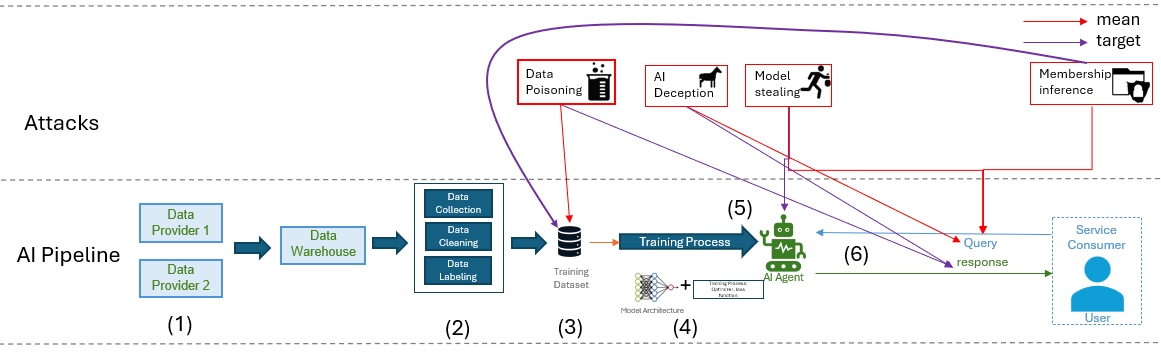
\includegraphics[width=\linewidth]{img/patas/attacks.png}
    \caption{Attack surface in the AI lifecycle pipeline, from data collection to model deployment.}
    \label{fig:attacks}
\end{figure}

\paragraph{Data Poisoning and Training-Time Attacks}
One of the most extensively studied threats is data poisoning, in which adversaries inject malicious or carefully crafted samples into the training dataset~\cite{chen2017targetedbackdoorattacksdeep}. Poisoned data may be mislabeled, backdoored, or statistically biased, causing the trained model to behave incorrectly under specific conditions while maintaining high performance on standard test sets. Such attacks are particularly dangerous because they undermine the assumption that training data faithfully represent the task domain. Standard performance metrics often fail to reveal poisoning effects, allowing compromised models to appear reliable.

\paragraph{Inference-Time Attacks and Model Exploitation}
Beyond training-time manipulation, deployed models are vulnerable to inference-time attacks. Model stealing or extraction attacks exploit repeated queries to reconstruct an approximation of the target model, threatening intellectual property and enabling subsequent adversarial attacks. Membership inference attacks aim to determine whether specific data points were part of the training dataset, raising serious privacy concerns. These attacks exploit overly confident predictions or memorization effects and demonstrate that model outputs can leak sensitive information even in the absence of explicit access to training data.

\paragraph{AI Deception and Strategic Manipulation}
More recently, attention has shifted toward AI deception, where adversarial agents deliberately manipulate inputs, interactions, or contextual information to induce misleading but seemingly plausible model outputs. Unlike classical adversarial examples, deceptive behaviors may not rely on imperceptible perturbations but instead exploit semantic ambiguity, contextual manipulation, or systematic bias in data sources. In multi-agent or human–AI interaction settings, deception may arise from untrusted information sources, colluding agents, or strategically misleading inputs designed to influence downstream decisions without triggering conventional anomaly detection mechanisms.

AI deception highlights a fundamental limitation of confidence-based reliability measures: a system may produce confident, well-calibrated predictions while being systematically misled. Detecting such behaviors requires reasoning not only about uncertainty, but also about the trustworthiness of evidence sources and the propagation of trust through the system.

\paragraph{Trust as a Lifecycle-Wide Concern}
Taken together, these attack classes illustrate that vulnerabilities in AI systems are not confined to a single stage of development. Trust can be compromised during data collection, labeling, training, evaluation, or deployment, and adversarial behavior may manifest long after a model has been trained. Consequently, the trustworthiness of a prediction cannot be viewed as a static property of a model alone, but must be understood as a dynamic property that depends on the provenance, quality, and interaction of data, model parameters, and operational context.

These observations motivate trust-aware frameworks that assess and propagate trust across the AI lifecycle, rather than relying solely on predictive accuracy or uncertainty estimates. Such frameworks aim to complement existing defenses by providing structured, evidence-centric reasoning about reliability and misuse, forming the foundation for the trust assessment approaches discussed in the subsequent sections.

\subsection{Training Dataset Quality and Trustworthiness}
\label{subsec:dataset_quality}

The quality and reliability of training datasets play a central role in determining the trustworthiness of neural network models. Since modern learning systems derive their behavior primarily from data rather than explicit rules, deficiencies in dataset construction can directly translate into systematic model failures. In safety-critical and high-assurance settings, dataset quality must therefore be treated as a first-class concern rather than an implicit assumption.

\paragraph{Data Poisoning and Dataset Trust}
One of the most direct threats to dataset trustworthiness is data poisoning, in which adversaries inject malicious, mislabeled, or carefully crafted samples into the training data. Poisoning attacks can subtly manipulate model behavior, for example by inducing targeted misclassifications or embedding backdoors, while preserving high accuracy on standard test sets. This makes poisoning particularly difficult to detect using conventional performance metrics and highlights a fundamental challenge: high predictive accuracy does not imply that the underlying training data are trustworthy.

More broadly, data poisoning illustrates that dataset trustworthiness is not a binary property but a matter of degree, dependent on the quality, provenance, and consistency of available evidence. Assessing dataset trust therefore requires reasoning under epistemic uncertainty, especially when dataset construction processes are opaque, distributed, or partially adversarial.

\paragraph{Ambiguity, Bias, and Epistemic Uncertainty in Datasets}
Beyond explicit attacks, even benign datasets may suffer from ambiguity, bias, and incomplete documentation. Meyer et al.~\cite{meyer2023multiplicity} emphasize that a single dataset can often support multiple valid interpretations of what it represents, due to unclear population coverage, subjective annotation choices, or undocumented filtering decisions. This multiplicity reveals an often-overlooked source of epistemic uncertainty in dataset evaluation: uncertainty about what claims a dataset actually supports.

Traditional approaches to dataset bias focus on statistical imbalance, demographic parity, or fairness metrics, often using resampling or reweighting techniques~\cite{10.1145/3600211.3604691,roy2022multi}. While effective for certain bias patterns, these methods typically assume that datasets are clean, fully labeled, and centrally accessible. In federated and decentralized learning settings, bias assessment becomes substantially more complex due to client heterogeneity, partition skew, limited metadata, and partial observability~\cite{roy2024fairness,electronics13234664}. Although mitigation strategies such as weighted aggregation or loss regularization have been proposed~\cite{electronics13234664}, existing work rarely quantifies confidence in the bias assessment itself when evidence is incomplete or noisy.

\paragraph{Dataset Evaluation Frameworks and Composite Trust Scores}
To improve transparency and accountability, several frameworks have been proposed to systematize dataset evaluation. Datasheets for Datasets~\cite{gebru2018datasheets} promote structured documentation of data collection, intended use, and known limitations. More recent scorecard-based approaches, such as METRIC~\cite{schwabe2024metric} and FRIES~\cite{10.1007/978-3-031-63787-2_15}, aggregate expert assessments across multiple quality dimensions, including fairness, robustness, and safety.

While these frameworks represent important progress, they largely rely on deterministic expert judgments and assume the availability of complete and reliable metadata. They do not provide formal mechanisms to represent uncertainty, disagreement, or missing evidence, nor do they distinguish between a low trust score and low confidence in the assessment itself. As a result, confidence in dataset evaluation cannot be explicitly reasoned about or propagated.

\paragraph{Annotation Noise and Trust in Labels}
Annotation quality is a critical component of dataset trustworthiness, particularly in supervised learning. Inter-annotator agreement metrics such as Cohen’s Kappa are commonly used to summarize labeling consistency, but these metrics provide only coarse, global measures and obscure instance-level uncertainty.

A substantial body of work on crowd annotation modeling addresses noisy labels by inferring latent ground truth. The seminal Dawid--Skene model~\cite{dawid1979maximum} estimates annotator-specific confusion matrices using expectation--maximization. Subsequent extensions such as GLAD~\cite{whitehill2009whose} incorporate annotator expertise and item difficulty, while MACE~\cite{hovy2013learning} focuses on identifying unreliable or adversarial annotators. Although effective for label denoising, these approaches ultimately collapse disagreement into point estimates of labels or annotator competence, discarding residual uncertainty.

More recent work has applied Subjective Logic to preserve and reason about annotation uncertainty. Subjective Logic Encodings (SLEs)~\cite{SLencodings,vasilakes2025sle} represent inter-annotator disagreement as belief--disbelief--uncertainty triplets, enabling instance-level trust assessment that explicitly distinguishes consensus from ignorance. This perspective aligns with the view that annotation disagreement is not merely noise to be eliminated, but evidence to be interpreted.

\paragraph{Toward Uncertainty-Aware, Data-Centric Trust Assessment}
Subjective Logic has also been applied more broadly to trust assessment in AI systems, including model-level trust~\cite{wang2020there}, evaluation metrics~\cite{10.1145/3605098.3635966}. However, most existing approaches remain model-centric or metric-centric and do not address dataset-level properties such as representativeness, bias, or sampling quality in a unified manner.

Taken together, existing approaches to dataset quality assessment either emphasize qualitative documentation without formal uncertainty modeling, deterministic composite scores without confidence representation, or trust modeling applied to isolated components of the data pipeline. What remains missing is a unified framework that integrates heterogeneous evidence, annotation reliability, bias assessment, and explicit uncertainty reasoning into a coherent evaluation of dataset trustworthiness. Addressing this gap is essential for trustworthy neural-network training and motivates the data-centric trust modeling approaches developed in this thesis.


\section{Synthesis and Gap Summary}
\todo[inline]{Estimated Nb Pages: 1}